\documentclass[diplom,german]{hgbthesis}

\usepackage{geometry}
\usepackage{titlesec}
\usepackage{pdfpages}
\geometry{a4paper,left=30mm,right=30mm, top=2cm, bottom=2cm}

\bibliography{bibliography}

\graphicspath{images/}

%--------surpress chapter headings 'Chapter N'----------
\titleformat{\chapter}[display]
{\bfseries\huge}                                            
{\filright}
{1ex}{}[]

\begin{document}

\title{KTI - Kapsch Tablet Infrastructure}
\logofile{Images/kti_logo}
\author{Götze Sebastian, Hammer Samuel, Kaufmann Michael, Müller Konstanze, Steinhäuser 				Philip}
\studiengang{Höhere Lehranstalt für Informatik}
\studienort{HTBLVA Spengergasse Wien 5}
\abgabedatum{2015}{05}{15}

%\maketitle
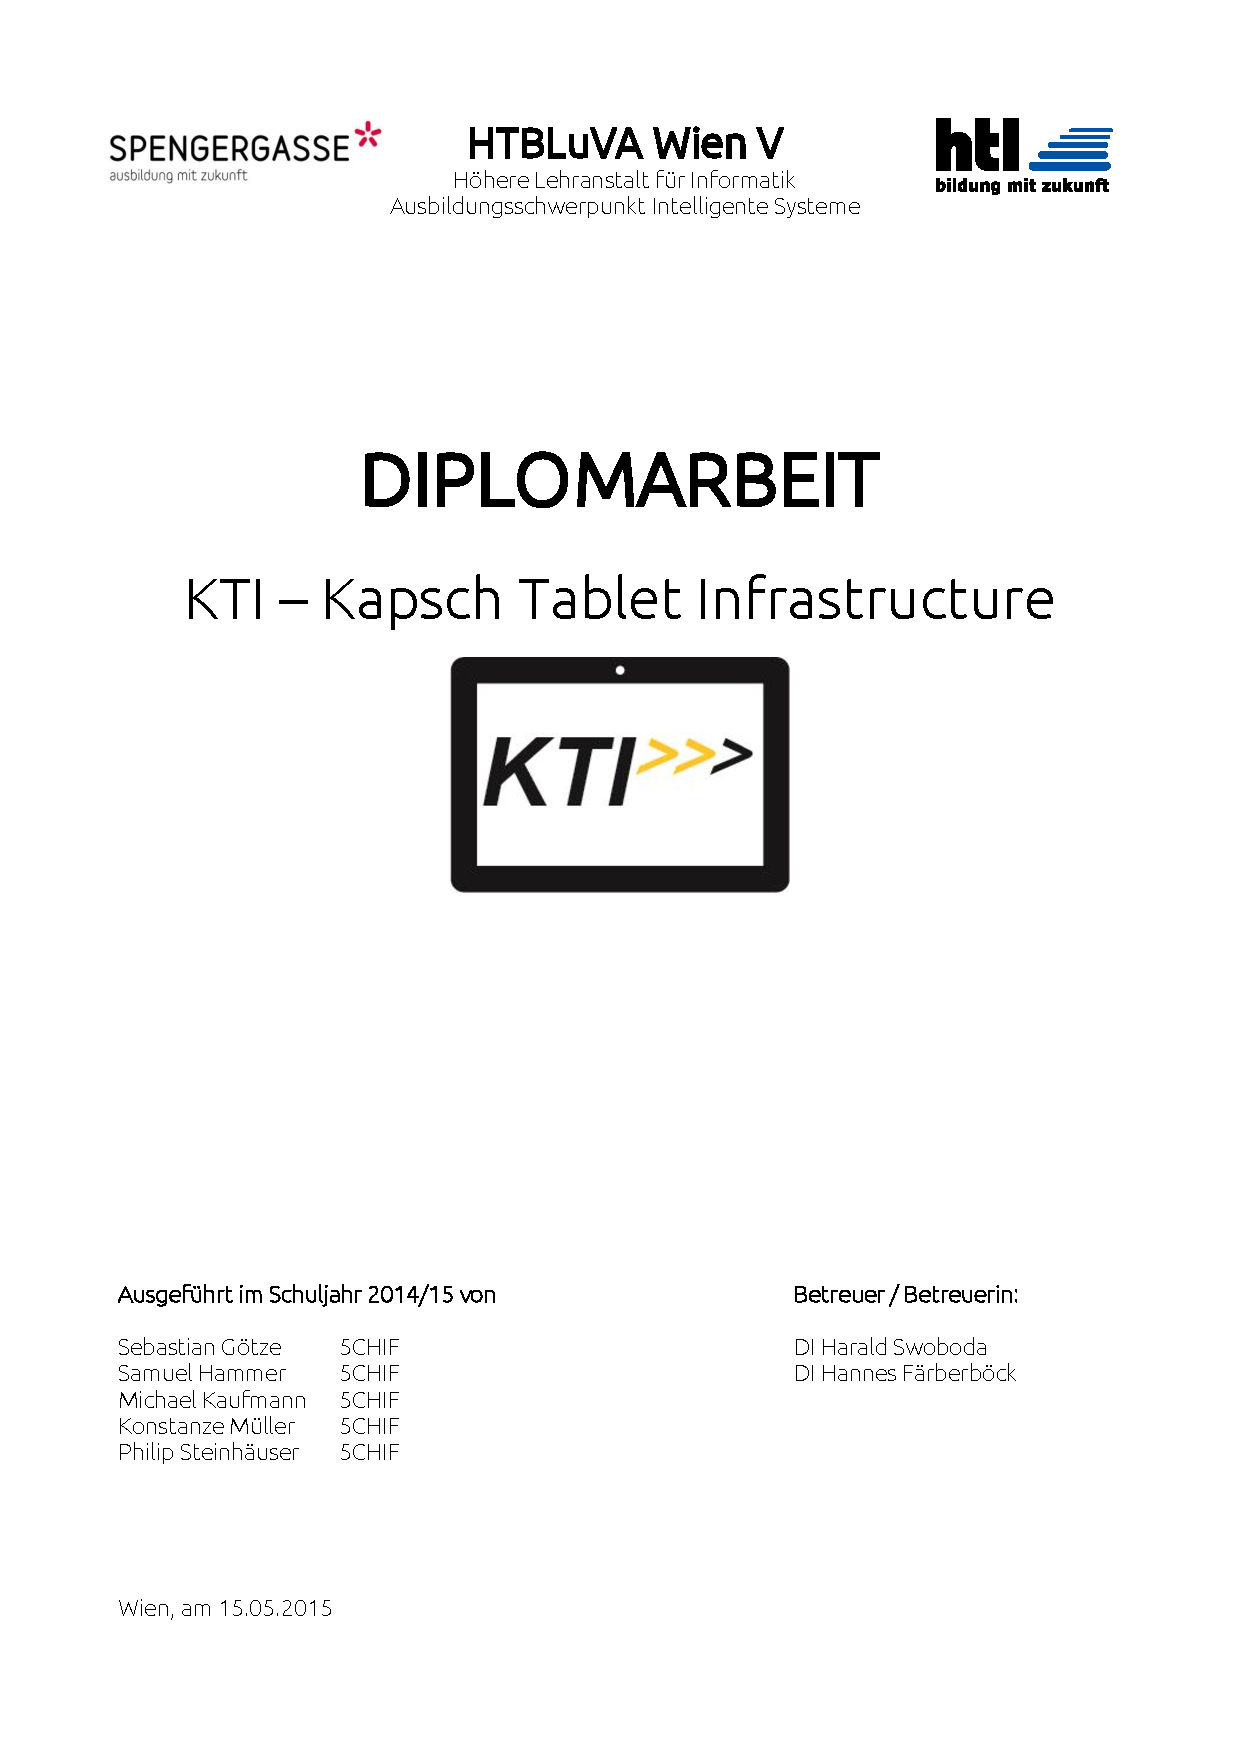
\includepdf{da_titelseite}

\frontmatter
\section*{}
\newpage
\thispagestyle{empty}
\chapter*{Kurzfassung}
\section*{Aufgabenstellung}
Die Aufgabe von Kapsch an das Projektteam ist es, verschiedene Softwarelösungen zum Systemschutz von Android-Tablets zu testen. Dazu soll ein Untersuchungsbericht angefertigt werden. In diesem werden die Ergebnisse  festgehalten und verglichen, um das beste System für die Kunden von Kapsch zu ermitteln. Ein Prototyp in Form eines Android-Tablets ist ebenfalls zu erstellen. Dieser soll mit dem besten, aus dem Untersuchungsbericht hervorgegangenen, Schutzsystem ausgestattet sein.
\section*{Realisierung}
Die Firma Kapsch wünscht einen Untersuchungsbericht, aus dem hervorgeht, welcher Systemschutz für Android-Tablets am besten für spezifische Kunden geeignet ist. In diesem Bericht werden zwei bis drei verschiedene Systeme zur Absicherung eines Android-Tablets verglichen. Darin wird auf die Vor- und Nachteile des jeweiligen Systems eingegangen, sowie auf das Fehlen von Funktionen aufmerksam gemacht. Dies ermöglicht dem Auftraggeber das bestmögliche System für seine Kunden zu ermitteln.
\section*{Ergebnisse}
Neben dem Untersuchungsbericht wird zusätzlich ein Tablet als Prototyp abgeliefert. Dieses Tablet ist mit dem Schutzsystem ausgestattet, welches aus dem Untersuchungsbericht als am empfehlenswertesten hervorgeht.
\newline Am Ende des Projekts stehen 2 Endprodukte. 
\subsection*{Der Untersuchungsbericht}
Er vergleicht zwei bis drei Softwarelösungen zur Absicherung von Tablets. Pro Lösung müssen ihre Vor- und Nachteile vorhanden sein, sowie auch das Fehlen von Einstellungsmöglichkeiten. 

Am Ende des Untersuchungsberichts hat ein Vergleich der Systeme zu stehen, aus dem hervorgeht, welches nach der Meinung des Projektteams eingesetzt werden sollte. Dies muss mit Argumenten bekräftigt werden.
\newpage
\subsection*{Der Prototyp}
Der Prototyp ist ein Android-Tablet, welches auf die Anforderungen eines Beispielunternehmens zugeschnitten ist. Dabei sollen nur bestimmte Aktionen möglich sein. 
\begin{itemize}
	\item Nutzung von drei bestimmten Apps
	\item Kein Zugang zu den Einstellungen
	\item Keine Verbindung mit einem Computer möglich
	\item Kein Download von Apps, Fotos, Videos, etc.
	\item Kein Verlassen der gesicherten Umgebung
\end{itemize}

\newpage

\chapter*{Abstract}
\section*{Assignment of Tasks}
Our project partner Kapsch provides enterprise grade solutions for major operating systems such as Microsoft Windows 8. Due to the consumerization trend in industry platforms like Apple iOS and Android OS are on the rise in enterprise applications and leading system integrators like Kapsch are in need to understand those platforms, their applications and limitations. Based on experience and results from existing projects Kapsch has realized that for certain applications or scenarios the Apple iOS platform has its limitations and drawbacks. In particular industrial applications have a need for a rock-solid platform which enables a system integrator like Kapsch to operate a 24/7 application and service. So Kapsch is keen to expand their knowledge and experience towards the Android platform to be able to provide solution platform for industrial applications.
Aim of this cooperation is to co-work on a set of different feasibility concepts for realizing such a platform based on Android.
\section*{Realisation}
The company Kapsch wants an investigation report, which shows which system protection is suitable for Android tablets best for specific customers. In this report, two to three different systems to secure a Android tablets are compared. It takes into account the advantages and disadvantages of each system, as well as draw attention to the lack of features. This allows the customer the best possible system for its customers to determine.
\section*{Results}
In addition to the investigation report a tablet is delivered as a prototype. This tablet is equipped with the protection system, which is apparent from the investigation report as most recommendable.
\newline At the end of the project, there are two final results:
\subsection*{The Research Paper}
It compares two to three software solutions for securing tablets. For each solution, advantages and disadvantages must be present. As well as the lack of configuration options.

At the end of the investigation report, a comparison of the systems has to stand, out of the proceeds, which should be in accordance with the opinion of the project team used. This must be confirmed with arguments.
\newpage
\subsection*{The Prototype}
An Android tablet that is tailored to the requirements of a model company. It should be possible only certain actions.
\begin{itemize}
	\item Use of three specific apps
	\item No access to the settings
	\item No connection to a computer possible
	\item No downloading of apps, photos, videos, etc...
	\item Leaving the secure environment not possible
\end{itemize}

\newpage

\setcounter{tocdepth}{5}
\setcounter{secnumdepth}{5}
\tableofcontents

\mainmatter
\setcounter{page}{1}
\chapter{Einleitung}
\section{Motivation}
Im zunehmenden Maße finden sich mobile Endgeräte (z.B. Tablet) als Marketing-,\newline Informations- und Imageelement, aber auch als Teil von Prozessen im Retail- als auch im Industrieumfeld wieder. Diese ersetzen oder erweitern bestehende Lösungen (z.B. Kiosk, Digital-Signage, Laptops, Industrie PCs) um interaktive Elemente und unterstützen so Unternehmen in ihren Geschäftsprozessen. 
Bei der eingesetzten Lösung ist es aus Sicht des Retail und Industriekunden wichtig, die Handhabung und das Erlebnis des Gerätes für den Anwender zu erhalten. Die Einsatzgebiete reichen dabei von Tablets in Produktionsprozessen zu Zwecken der Qualitätssicherung (eigene Applikationen mit Dokumentationsfunktionen) bis hin zu Multimedia-Terminals im stationären Handel. Um diese verschiedenen Szenarien realisieren zu können, ist es notwendig eine stabile, sichere und wartbare Plattform zu konstruieren, die zum einen die Anwendung in unterschiedlichen Einsatzgebieten ermöglicht und zum anderen für den Betriebsführer leicht bereitzustellen und zu warten ist.
\paragraph*{}
Um den hier angeführten allgemeinen Anforderungen ihrer Kunden gerecht zu werden, benötigt Kapsch die passendste Softwarelösung im Bereich Security für die hierfür in Betracht gezogenen Tablets. Um diese Softwarelösung zu ermitteln, wurde ein Projektteam des fünften Jahrgangs der HTBLVA Spengergasse, Fachbereich Informatik, mit der Aufgabe der Eroierung dieser Lösung und  der Erstellung eines Konzepts betraut. Das Projekt KTI – Kapsch Tablet Infrastructure wird von dem Projektmanager Philip Steinhäuser geleitet  und besteht aus den Teammitgliedern Sebastian Götze, Samuel Hammer,\newline Michael Kaufmann und Konstanze Müller. Das Projektteam steht in engem Kontakt mit dem Project owner, welcher durch die Mitarbeiter Bernhard Bruckner und Jürgen Krammer vertreten ist. 
\paragraph*{}
Kapsch unterstützt das Projekt mit diversen Hilfeleistungen sowie Technischer Supports, intellektueller Hilfe und finanzieller Unterstützung beim Kauf des Tablets, welches nach Beendigung des Projekts wieder in den Besitz von Kapsch übergehen wird.

\newpage

\section{Projektpartner}
\begin{figure}[H]

\includegraphics[scale=1.0]{Images/kapsch_logo}
\caption{Kapsch Logo}
\end{figure}
Die Kapsch Group setzt sich aus 3 Hauptunternehmen zusammen:
\begin{itemize}
	\item Kapsch TrafficCom
	\item Kapsch CarrierCom
	\item Kapsch BusinessCom
\end{itemize}

\paragraph*{}
Die Kapsch TrafficCom ist internationaler Anbieter von Technologien, Lösungen und Dienstleistungen für den Intelligent Transportation Systems (ITS) Markt. 
\paragraph*{}
Die Kapsch CarrierCom ist globaler Lösungspartner für Telco-Carrier und Communication-Provider sowie Railway-Operator. 
\paragraph*{} 
Unser konkreter Projektpartner ist die Kapsch BusinessCom.
Mit 1.400 Mitarbeitern, einem Umsatz von knapp 300 Millionen Euro und Niederlassungen in Österreich, Tschechien, Slowakei, Ungarn, Rumänien und Polen positioniert sich das Unternehmen als einer der führenden ICT-Servicepartner in Zentral- und Osteuropa. Kapsch setzt auf Partnerschaften mit führenden Branchengrößen wie Apple, Cisco, Google, HP oder Microsoft, um seinen rund 17.000 Kunden den bestmöglichen Service gewährleisten zu können.

\newpage

\section{Ursprungsproblem}
Die Aufgabe von Kapsch an das Projektteam ist es, verschiedene Softwarelösungen zum Systemschutz von Android-Tablets zu testen. Die vom Project owner zum Test gewünschten Softwarelösungen sind.
\begin{itemize}
	\item MDM
	\item MDM + Container
	\item Samsung Knox
\end{itemize}
Zusätzlich besteht noch die Möglichkeit einer \textbf {Linux Manipulation}, welche jedoch für Kapsch aus rechtlichen Gründen nicht in Frage kommt, da diverse Garantieverletzungen auftreten und zusätzlich enorme Kosten aufgrund von hohen Entwicklungskosten und langen Entwicklungszeiten, bis das System einwandfrei funktioniert, anfallen würden.
\paragraph*{}
Zu diesen Schutzsystemmöglichkeiten soll ein Untersuchungsbericht angefertigt werden. In diesem werden die Ergebnisse  festgehalten und verglichen, um das beste System für die Kunden von Kapsch zu ermitteln.
\paragraph*{}
Auf Basis dieses Untersuchungsberichts soll dann die passendste Softwarelösung ausgewählt werden, welche in ein Konzept eingebaut wird. Ein Teil dieses Konzepts beinhaltet die Implementierung der ausgewählten Softwarelösung auf ein Tablet, welches dann als Prototyp deklariert wird. 
\paragraph*{}
Der Untersuchungsbericht in Kombination mit dem Prototyp ist das Ergebnis, welches über den Ausgang dieses Projekts entscheidet.


\section{Vorgehensweise}
\subsection{Vorbereitung}
\begin{itemize}
	\item Vorbereitungsmeeting mit Kapsch
	\item Einlesen in Technologie
	\item Erste Recherchen
\end{itemize}
\subsection{Planung}
\begin{itemize}
	\item Projektantrag
	\item Vorstudie
	\item PSP (Projektstrukturplan)
	\item OSP (Objektstrukturplan)
	\item Timetable bzw. Gantt-Chart
	\item Lastenheft
	\item Pflichtenheft
	\item Projekthandbuch
	\item Checklist Template
	\item Research Template
	\item Untersuchungsbericht
	\item Diplomarbeit
\end{itemize}
\subsection{Durchführung}
\begin{itemize}
	\item Recherche
	\item Erstellung des Untersuchungsberichtes
	\item Auswahl der passenden Lösung
	\item Konzept erstellen
	\item Ausgewählte Lösung in Konzept einarbeiten
	\item Konzept teilweise umsetzen - Konfiguration der Lösung auf Tablet (Prototyp)
\end{itemize}
\subsection{Ergebnis}
\begin{enumerate}
	\item Untersuchungsbericht
	\item Prototyp
\end{enumerate}

\subsection{Organigramm}
\begin{figure}[H]
	\centering
	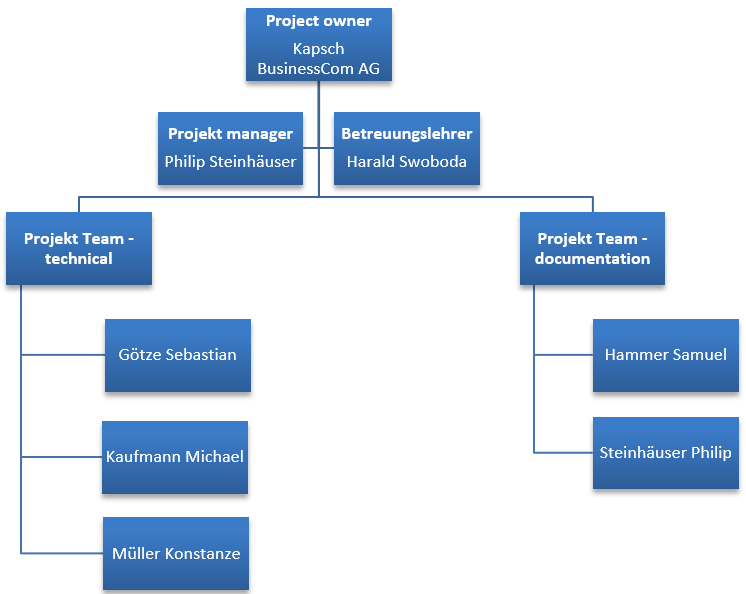
\includegraphics[scale=0.6]{Images/organigramm}
	\caption{Projekt-Organigramm}
\end{figure}
Die Aufgaben des Projekts wurden so verteilt, dass das Dokumentationsteam sämtliche Projektmanagementaufgaben und das Technikteam alle Research- und Testungsaufgaben übernimmt.
\begin{figure}[H]
	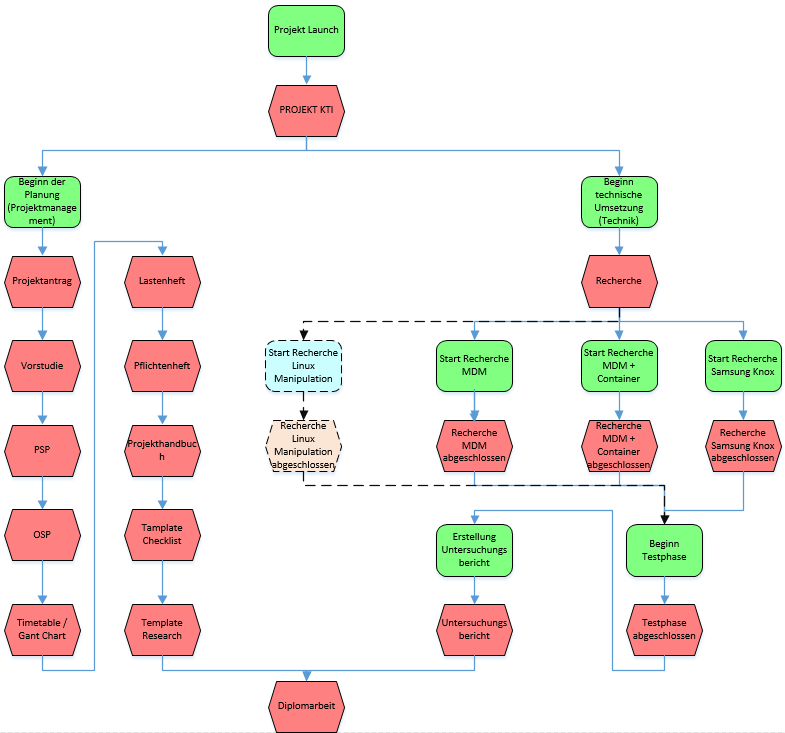
\includegraphics[scale=0.7]{Images/arbeitsteilung}
	\caption{Aufgabenverteilung - Diagramm}
\end{figure}
Dieses Ablaufdiagramm zeigt auf der einen Seite die Reihenfolge der erstellten Dokumente, so wie beispielsweise, dass der OSP und der Timetable/Gantt Chart auf dem PSP aufbaut, da dieser zuvor erstellt wurde und diese drei Dokumente konsistent sein müssen.
\paragraph*{}
Auf der Technik Seite wiederum sieht man, dass zuerst eine umfangreiche Recherche nötig ist bzw. war, bevor die Wahl der passendsten Softwarelösung getroffen werden kann/konnte, welche dann schlussendlich für das Konzept und in weiterer Folge für die Konfiguration des Prototyps verwendet werden konnte/wurde.


\newpage

Wenn man sich unsere Vorgehensweise nun Schritt für Schritt auf die beiden Sub Teams aufgeteilt anschauen würde, würde folgendes Bild entstehen:

\begin{table}[H]
	\begin{tabular}{| c | p{6.5cm} | p{7.5cm} |}
		\hline
		\textbf \# & \textbf{Dokumentation} & \textbf{Technik}
		\\\hline %----------new line----------
		1 
		&%-----
		\begin{itemize}
			\item Erstellung des Projektantrages
			\item Erstellung der Vorstudie
			\item Erstellung PSP
			\item Erstellung OSP
		\end{itemize}
		&%-----
		-
		\\\hline %----------new line----------
		2
		&%-----
		\begin{itemize}
			\item Erstellung des Gantt-Chart
			\item Erstellung Lastenheft
			\item Erstellung Pflichtenheft
		\end{itemize}
		&%-----
		\begin{itemize}
			\item Beginn der Recherchephase
			\begin{itemize}
				\item Recherche Linux Manipulation
				\item Recherche MDM
				\item Recherche MDM+Container
				\item Recherche Samsung Knox
			\end{itemize}
		\end{itemize}
		\\\hline %----------new line----------
		3
		&%-----
		\begin{itemize}
			\item Erstellung Projekthandbuch
			\item Erstellung Research Template
			\item Erstellung Checklist Template
		\end{itemize}
		&%-----
		\begin{itemize}
			\item Festhalten der Rechercheergebnisse in Templates
			\item Recherchephase abgeschlossen
			\begin{itemize}
				\item Recherche Linux Manipulation abgeschlossen
				\item Recherche MDM abgeschlossen
				\item Recherche MDM+Container abgeschlossen
				\item Recherche Samsung Knox abgeschlossen
			\end{itemize}
		\end{itemize}
		\\\hline %----------new line----------
		4
		&%-----
		\begin{itemize}
			\item Erstellung Diplomarbeit
		\end{itemize}
		&%-----
		\begin{itemize}
			\item Beginn der Testphase
			\item Erstellung des Untersuchungsberichts
		\end{itemize}
		\\\hline %----------new line----------
		5
		&%-----
		\begin{itemize}
			\item Fertigstellung Diplomarbeit
			\item Fertigstellung Projekthandbuch
		\end{itemize}
		&%-----
		\begin{itemize}
			\item Abschluss der Testphase
			\item Fertigstellung des Untersuchungsberichts
		\end{itemize}
		\\\hline %----------new line----------
	\end{tabular}
	\caption{Projektablauf}
\end{table}

\newpage

\section{Arbeitsaufteilung}
In unserem Projekt wurde die Arbeit so aufgeteilt, dass kein Teammitglied zu viel oder zu wenig, sondern genau richtig ausgelastet ist, um die Freude und Motivation an der Arbeit über die Dauer der Projektarbeit immer konstant hoch zu halten. Hier zu sehen ist, was welches Projektmitglied an welchem Dokument gearbeitet hat oder welche Softwarelösung von ihm recherchiert und textuell beschrieben wurde.

\subsection{Sebastian Götze}
Sebastian war Verantwortlicher für die Recherche an den Softwarelösungen Mobile Device Management sowie Linux Manipulation, welches jedoch lediglich aus Informationszwecken, und nicht aufgrund seiner Verwendung recherchiert wurde. Weiters arbeitete er an Dokumenten wie dem Projektantrag, der Vorstudie, dem Pflichtenheft sowie dem Projekthandbuch mit. Von ihm stammen außerdem das Checklist Template sowie das Research Template, welche für die Recherche sowie das Testing der einzelnen Softwarelösungen verwendet wurden.
%	\begin{itemize}
%		\item Projektantrag
%		\item Vorstudie
%		\begin{itemize}
%			\item status quo
%			\item MDM
%		\end{itemize}
%		\item Template Checklist
%		\item Template Research
%		\item Pflichtenheft
%		\begin{itemize}
%			\item Unternehmensperspektive
%			\item Funktionale Beschreibung
%		\end{itemize}
%		\item Projekthandbuch
%		\begin{itemize}
%			\item Project Assignment
%			\item Plan of objects of consideration
%			\item Project Work-Package Specification
%			\item Project Rules
%		\end{itemize}
%		\item Gantt-Chart
%		\item Mobile Device Management (MDM)
%		\begin{itemize}
%			\item Recherche
%			\item Testing
%			\item Untersuchungsbericht
%			\item Diplomarbeit
%		\end{itemize}
%		\item Linux Manipulation
%		\begin{itemize}
%			\item Recherche
%			\item Untersuchungsbericht
%			\item Diplomarbeit
%		\end{itemize}
%		\item Prototyp
%	\end{itemize}


\subsection{Samuel Hammer}
Samuel war Verantwortlicher für das Erstellen sämtlicher Präsentationen sowie für die Schriftführung bei unseren Projectownermeetings, welche im Anschluss an diese von ihm in Form von Besprechungsprotokollen dokumentiert und festgehalten wurden. Weiters arbeitete er am Projektantrag, der Vorstudie, dem Projekthandbuch, dem Pflichtenheft sowie der Diplomarbeit mit. Von ihm stammt außerdem die erste Version unserer Zeitplanung in Form eines Gantt Charts, welche bzw. welches als Grundlage für die folgenden Versionen und als Unterstützung der Planung von etwaigen Terminen von Abgaben, sowie zur Projektfortschrittskontrolle verwendet wurde.
%	\begin{itemize}
%		\item Projektantrag
%		\item Vorstudie
%		\begin{itemize}
%			\item Critical Appraisal
%			\item Android Technology Analysis
%		\end{itemize}
%		\item Projekthandbuch
%		\begin{itemize}
%			\item Project Assignment
%			\item Description of Pre- and Post-Project Phase
%			\item Project Work-Package Specification
%			\item Project Bar Chart
%			\item Minutes - Project Co-Ordination
%		\end{itemize}
%		\item Pflichtenheft
%		\begin{itemize}
%			\item Funktionen
%			\item Betriebsbedingungen
%			\item Härtung der mobilen Endgeräte
%		\end{itemize}
%		\item Besprechungsprotokolle
%		\item Präsentationen
%		\begin{itemize}
%			\item Statuspräsentationen
%			\begin{itemize}
%				\item 09.12.2014
%				\item 08.01.2015
%				\item 19.02.2015
%				\item 19.03.2015
%				\item 16.04.2015
%			\end{itemize}
%			\item Abschlusspräsentation Englisch
%			\item Abschlusspräsentation Deutsch
%		\end{itemize}
%		\item Gantt-Chart
%		\item Diplomarbeit
%	\end{itemize}

\subsection{Michael Kaufmann}
Michael war Verantwortlicher für die Recherche an der Softwarelösung Samsung Knox, sowie deren Implementierung nach Beendigung der Research- und Testingphase. Weiters arbeitete er am Projektantrag, der Vorstudie, dem Projekthandbuch sowie dem Pflichtenheft mit. Zudem sind von ihm Gantt-Chart Versionen, welche eine große Rolle in der Planung und dem reibungslosen Ablauf unseres Projekts spielten, erstellt worden.
%	\begin{itemize}
%		\item Projektantrag
%		\item Vorstudie
%		\begin{itemize}
%			\item Samsung Knox
%		\end{itemize}
%		\item Projekthandbuch
%		\begin{itemize}
%			\item Project assignment
%			\item Project Objectives
%			\item Project Work-Package Specification
%		\end{itemize}
%		\item Pflichtenheft
%		\begin{itemize}
%			\item System Architecture
%			\begin{itemize}
%				\item Hardware
%				\item Software
%			\end{itemize}
%		\end{itemize}
%		\item Gantt-Chart
%		\item Samsung Knox
%		\begin{itemize}
%			\item Recherche
%			\item Testing
%			\item Untersuchungsbericht
%			\item Diplomarbeit
%			\item Implementierung
%		\end{itemize}
%		\item Prototyp
%	\end{itemize}

\subsection{Konstanze Müller}
Konstanze war Verantwortliche für die Recherche der Softwarelösung Mobile Device Management mit Container, bei welcher sie einige für den später erstellten Untersuchungsbericht relevante Daten sammeln und textuell in den jeweiligen Checklist und Research Templates festhalten konnte. Weiters arbeitete sie an dem Projektantrag, der Vorstudie, dem Projekthandbuch sowie dem Pflichtenheft mit. Gemeinsam mit Philip erstellte sie alle zwei Wochen einen Statusbericht.
%	\begin{itemize}
%		\item Projektantrag
%		\item Vorstudie
%		\begin{itemize}
%			\item MDM + Container
%		\end{itemize}
%		\item Projekthandbuch
%		\begin{itemize}
%			\item Project Assignment
%			\item Project environment Graphic
%			\item Project Environment Table
%			\item Project Work-Package Specification
%			\item Project Risk Analysis
%			\item Project Status Reports
%		\end{itemize}
%		\item Pflichtenheft
%		\begin{itemize}
%			\item Target Groups
%			\item Quality Criteria
%		\end{itemize}
%		\item Besprechungsprotokolle
%		\item Statusberichte
%		\item Mobile Device Management (MDM) + Container
%		\begin{itemize}
%			\item Recherche
%			\item Testing
%			\item Untersuchungsbericht
%			\item Diplomarbeit
%		\end{itemize}
%		\item Prototyp
%	\end{itemize}

\newpage

\subsection{Philip Steinhäuser (Projektleiter)}
Philip war neben seiner Tätigkeit als Projektleiter auch Verantwortlicher für das Projekthandbuch, die Meilensteintrendanalyse, die Statusberichte, das Abnahmeprotokoll sowie für das Project Controlling und Zeitmanagement des Projekts.  Er arbeitete am Projektantrag, der Vorstudie, dem Objektstrukturplan (OSP), dem Projektstrukturplan (PSP), dem Pflichtenheft, dem Projekthandbuch sowie der Diplomarbeit mit. Von ihm wurde weiters die eben schon erwähnte Meilensteintrendanalyse sowie das Abnahmeprotokoll verfasst. Weiters zählte die regelmäßige Aktualisierung des Projekthandbuchs sowie die Vertretung des Projektteams gegenüber dem Projektpartner und den Lehrern zu seinen Aufgaben. 
%\begin{itemize}
%	\item Projektantrag
%	\item Vorstudie
%	\begin{itemize}
%		\item Management Summary
%		\item Task
%		\item SWOT - Analyse
%	\end{itemize}
%	\item Gantt-Chart
%	\begin{itemize}
%		\item laufende Aktualisierung und Projektfortschrittskontrolle
%	\end{itemize}
%	\item Kooperationsvereinbarung
%	\item Meilensteinplan
%	\item Meilensteintrendanalyse
%	\item Objektstrukturplan - OSP
%	\item Projektstrukturplan - PSP
%	\item Pflichtenheft
%	\begin{itemize}
%		\item Requirement Specification
%		\item Embedding in Organisation
%		\item Milestones
%	\end{itemize}
%	\item Projekthandbuch
%	\begin{itemize}
%		\item Project Assignment
%		\item Project Organisation Chart
%		\item Project Organisation
%		\item Work Breakdown Structure (WBS)
%		\item Project Work-Package Specification
%		\item Milestoneplan
%		\item Project Communication
%		\item Project Responsibility Matrix
%		\item Project Documentation
%		\item Project Co-Ordination
%		\item Project Status Report
%		\item Laufende Aktualisierung und Ausarbeitung des einzelnen Punkte des Projekthandbuchs
%	\end{itemize}
%	\item Statusberichte
%	\item Abnahmeprotokoll (Acceptance Testing Protocol - ATP)
%	\item Diplomarbeit
%\end{itemize}
\chapter{Studie}
\section{Android}
Android ist, im Gegensatz zu anderen mobilen Betriebssystemen auf dem Markt, eine offene Plattform. Das kommt im Wesentlichen daher, dass Android auf einem open source System, dem Linux Kernel, aufbaut. Durch die freie Verfügbarkeit des Codes gibt es im Android-Bereich eine große Developer-Szene, die laufend eigens modifizierte Betriebssysteme (ROMs) und Apps hervorbringt.
Ein so hoher Grad an Offenheit birgt jedoch auch gewisse Sicherheitsrisiken und öffnet Angriffsvektoren. Um diese Gefahren besser zu verstehen, sollte man sich eingehend mit der Android Architektur und dem darin enthaltenen Sicherheitskonzept befassen.

\subsection{Architektur}
\begin{figure}[H]
\centering
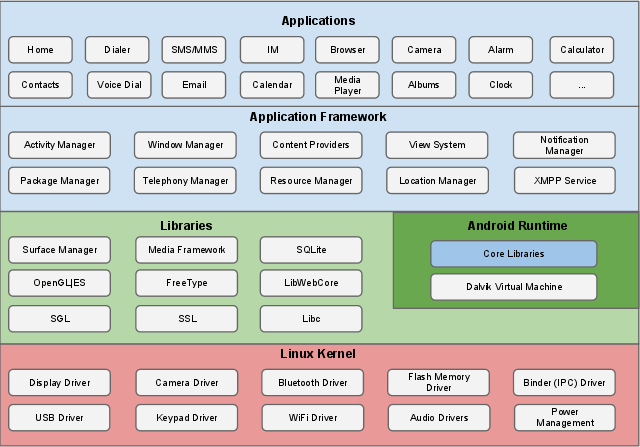
\includegraphics[scale=0.7]{Images/android_stack}
\caption{Android Systemarchitektur}
\end{figure}
Wie in Abbildung 1 zu sehen ist, bildet der Linux Kernel die unterste Schicht der Architektur. Auf ihm baut das gesamte Betriebssystem mitsamt aller Sicherheitskonzepte auf. Der Kernel stellt die Brücke zwischen Hard- und Software dar und enthält die Treiber für diverse andere Komponenten eines Smartphones, wie beispielsweise Modem, GPS Empfänger, Kamera, etc. 
\paragraph*{}
In der darüber liegenden Ebene sind die Android Libaries sowie die Runtime, also die „Dalvik Virtual Machine“, zu finden. \newline
Android Apps sind meist in Java programmiert und werden jeweils in einer eigenen virtuellen Maschine ausgeführt, der DVM\footnote{Dalvik Virtual Machine}. Diese Systematik ermöglicht das logische, parallele, unabhängige Ausführen von verschiedenen Apps mit verschiedenen Benutzerrechten.
Die Libaries steuern und kontrollieren im Wesentlichen die Funktionen des Kernels und sind für die zentralen Funktionalitäten auf niedriger Ebene zuständig.
\paragraph*{}
Die nächsthöhere Ebene bildet das Application Framework. Hier befinden sich die Grundfunktionen von Android, wie zum Beispiel Telefonie, Location Services, Window Manager, Notification Manager, etc… 
Auf dieser Ebene werden Entwicklern äußerst umfangreiche APIs für das Entwickeln von Benutzeranwendungen (Apps) zur Verfügung gestellt.
\paragraph*{}
Die oberste Schicht in der Android-Systemarchitektur sind die Applikationen, welche der Benutzer selbst installiert und auf den darunterliegenden Schichten aufbaut.
\paragraph*{}
Dieser gesamte „Stack“ (=Stapel) wird in einem ROM zusammengefasst und auf ein Smartphone installiert. Durch die zuvor erwähnte Offenheit des Systems können so durch Modifizieren eines ROM Paketes stark angepasste Versionen von Android entwickelt und verwendet werden.


\subsection{Security}
Android wird als Betriebssystem mittlerweile auf ca, 84 \% aller Smartphones weltweit eingesetzt.\footnote{Link: http://www.idc.com/prodserv/									smartphone-os-market-share.jsp, Stand 10.11.2014} Ein Betriebssystem mit einem so großen Marktanteil erfordert ein durchdachtes und ausgereiftes Sicherheitskonzept.
Die drei grundlegenden Sicherheitsobjekte sind:

\begin{itemize}
	\item Schützen von Benutzerdaten
	\item Schützen von Systemressourcen (inklusive Netzwerk)
	\item Bereitstellen von Applikationsisolation
\end{itemize}
Um diese Objekte zu erreichen, stehen eine Reihe von Security-Features zur Verfügung:
\begin{itemize}
	\item Robuste Security auf der OS Ebene durch den Linux Kernel
	\item Erforderliche Sandbox für alle Apps
	\item Sichere interprozess Kommunikation
	\item Application signing
	\item Application-defined and user-grated permissons
\end{itemize}

\subsubsection{System- und Kernel Security}
Der Linux Kernel stellt das Fundament von Android dar. Durch dessen langjährige Wartung und Weiterentwicklung hat dieser sich zu einem äußerst sicheren und weit verbreiteten Kernel entwickelt, welcher auch in sicherheitsempfindlichen Umgebungen eingesetzt wird.
\paragraph*{}
Der Linux Kernel stellt einige der wichtigsten Sicherheitsfunktionen zur Verfügung.
\begin{itemize}
	\item Ein benutzerbasiertes Rechtemodell
	\item Prozessisolation
	\item Mechanismus für sichere IPC\footnote{Interprozesskommunikation} 
	\item Die Möglichkeit potenziell gefährliche Teile des Kernels zu entfernen
\end{itemize}
Im Gegensatz zum normalen Linux, wo mehrere Anwendungen mit demselben Benutzer ausgeführt werden, weist Android jeder Applikation eine eigene User ID zu und führt diese mit eben diesem User in einem separaten Prozess aus.
Diese Vorgehensweise resultiert in einer „Kernel-level Application Sandbox“. Dadurch kann eine App von Haus aus mit keiner anderen App kommunizieren, sofern dies nicht explizit erwünscht ist. Standardmäßig können Apps auch nicht auf Dinge wie Standort, die Telefonie-Funktion etc. zugreifen, sondern müssen erst um die Erteilung der entsprechenden Benutzerrechte ansuchen. Die Tatsache, dass diese Sandbox-Systematik auf Jahrzehnte alter UNIX Technologie aufbaut, macht das System leicht überwachbar und transparent, jedoch gleichzeitig effizient.
\paragraph*{}
Speicherfehler führen in vielen Betriebssystemen zu groben Sicherheitsrisiken und sind in der Lage, die Sicherheit eines Gerätes komplett zu kompromittieren. Bei Android kann ein solcher Speicherfehler durch das Sandboxing aller Applikationen auf OS-Level keinen allzu großen Schaden anrichten, da eventueller Schadcode nur im Kontext einer bestimmten App, mit eingeschränkten Benutzerrechten ausgeführt werden kann.
\paragraph*{}
Selbstverständlich ist auch die Applikations-Sandbox nicht zu 100 \% sicher, möchte man diese aber knacken, so muss man es schaffen, den gesamten Linux Kernel zu kompromittieren.
	
\subsection{Angriffsvektoren}
Angriffsvektoren sind Pfade, um ein Security Konzept zu durchdringen und so Zugriff auf gesicherte Ebenen eines Systems zu erlangen. Gerade bei einem Mobilen Betriebssystem wie Android, ist es von besonderer Wichtigkeit, diese Gefahrenquellen zu kennen und soweit wie möglich zu eliminieren, da Geräte, welche auf Android laufen, einen Großteil der Zeit angeschaltet und mit dem Internet verbunden sind. \par
Ein weiterer Grund, warum besonders mobile Endgeräte Ziel solcher Attacken sind, ist die Tatsache, dass Daten auf einem Smartphone oder Tablet meist aktuell sind. So werden beispielsweise neue E-Mails immer sofort via push mail heruntergeladen und gespeichert. Auch sogenannte TAN Codes, welche sich in den letzten Jahren als Autorisierung-Methode für online Überweisungen etabliert haben und via SMS übertragen werden, machen Smartphones zu einem brauchbaren Ziel für Hacker.
\subsubsection{Social Engineering}
Social Engineering ist eine Methode unautorisiert an Daten zu gelangen, ohne dabei technische Änderungen am System vorzunehmen. Hierbei wird versucht, den User mit Hilfe von falschen Informationen dazu zu bringen das System zu verändern oder eine schädliche Datei herunter zu laden und dem Angreifer so selbst den Weg zu ebnen. Ein Beispiel für Social Engineering ist der sogenannte „ILOVEYOU Virus“. Dieser wurde via E-Mail verschickt und gab vor, ein Liebesbrief zu sein, sodass der Benutzer ihn öffnet und selbst ausführt.
Gegen das Prinzip des Social Engineerings gibt es kein brauchbares Gegenmittel, da es einzig und allein auf den Entscheidungen des Users aufbaut.
\newpage
\subsubsection{Drive-by Exploitation}
Diese Angriffsmethode macht sich Bugs in vorhandener Software zu Nutzen, um schadhaften Code auf dem Device auszuführen. Mit Hilfe solcher Bugs gelingt es dem Angreifer Code über beispielsweise eine Website auf das Gerät des Opfers herunterzuladen und dann auf dem Zielsystem auszuführen. Drive-by Exploitation ist vor allem auf Desktop PC Systemen weit verbreitet. Durch diverse Sicherheitsmechanismen von Android, wie das Sandboxing der Apps oder die DVM (Dalvik Virtual Machine), ist es auf solchen Geräten wesentlich schwieriger schadhaften Code auszuführen und so das System nachhaltig zu beschädigen. Nichtsdestotrotz gibt es auch auf Android eine große Anzahl an Apps, welche native Software-Bibliotheken verwenden und so angreifbar gegen Drive-by Exploitation sind.
\subsubsection{Phishing}
Phishing Attacken werden benutzt, um sensible Informationen wie Login Daten abzugreifen. Der Angreifer gibt sich dabei als offizielle Instanz aus und bewegt den Nutzer dazu seine Daten preiszugeben. Dies geschieht beispielsweise über eine gefälschte Website, welche gleich aussieht wie die echte Website, nur dass die eingegebenen Daten direkt an den Angreifer weitergeleitet werden. Phishing beinhaltet einige Aspekte des Social Engineerings, daher gibt es auch hier keine wirklich gute Möglichkeit solche Attacken zu verhindern. Auf Mobilen Geräten ist die Situation allerdings ein wenig anders, da es für die meisten online Services eine eigene App gibt, welche nur über den offiziellen App Store heruntergeladen werden kann. Daher verwenden nur wenige User die Website und laufen damit nicht Gefahr Ziel einer Phishing Attacke zu werden.



\chapter{Varianten}
%-------------------------------Linux Manipulation------------------------------------
\section{Linux Manipulation}
\subsection{Allgemein}
\paragraph*{}
Dieser Teil befasst sich mit der Veränderung des Grundsystems eines jeden Android Geräts. Dieses Grundsystem basiert auf dem Open Source Betriebssystem Linux und existiert dabei in einer für Mobilgeräte angepassten Form. In seiner Standardimplementation bietet es zwar einige Funktion zur Erhöhung der Gerätesicherheit, jedoch nicht genügend, um es in einem betrieblichen Umfeld einzusetzen. Da Linux ein Open Source System ist, darf der Source Code von jedem angesehen und nach eigenen Wünschen verändert werden. Und genau hier setzt die Methode der Linuxmanipulation an. In dem man den Source Code so verändert, dass bestimmte Teile des Betriebssystems unzugänglich gemacht oder verschlüsselt werden, ist es möglich den späteren Benutzer vor unabsichtlichen Änderungen am System zu bewahren, welche den reibungslosen Betrieb stören könnten. Das bedeutet, dass dadurch ein vollkommen an die Bedürfnisse des Kunden angepasstes Betriebssystem möglich wäre. Um sich einen besseren Eindruck davon zu verschaffen, wie diese Manipulationen letztendlich aussehen, lohnt es sich auf die diversen frei am Markt erhältlichen Derivate zu werfen. Bekannte Beispiele dafür wären:
\begin{itemize}
	\item CyanogenMod
	\item Android AOSP
	\item Paranoid Android
	\item Dirty Unicorns
	\item etc.
\end{itemize}
Zwar sind diese nicht mit securitytechnischen Absichten entwickelt worden, aber sie zeigen trotzdem auf was mit einer Menge an Entwicklungsaufwand möglich ist. Da aber durch die tiefgreifenden Eingriffe in das System eines Android Gerätes auch die Garantieansprüche verloren gehen, ist das Projektteam zu einem schnellen Fazit zu kommen.
\subsection{Schlussfolgerung}
Die Methode der Linuxmanipulation ist für die Zwecke der Kapsch leider absolut nicht einsetzbar dar sich bei ihr gewisse Konflikte bezüglich Garantieanspruch und Kosten ergeben. Zwar wären über diese Methode sämtliche Anforderungen an das Endprodukt erfüllbar, jedoch bedarf es dazu eines so großen Entwicklungsaufwands, dass dieser sich in einem dermaßen hohen Endkundenpreis niederschlagen würde, welcher von kaum einem Unternehmen zu bezahlen wäre. Denn nicht nur die Beschäftigung einer Vielzahl von Entwicklern über einen langen Zeitraum hinweg, sondern auch der anfallende Support für das Produkt würde sich selbst für ein großes Unternehmen wie Kapsch nicht rentieren. Ein weiteres großes Manko dieser Methode ist die verfallende Garantie für die Hardware. Egal mit welchen Android Tablet diese Software ausgeliefert werden würde, sobald eine Veränderung der darauf vorinstallierten Software stattfindet, gehen sämtliche Garantieansprüche an den Hersteller verloren. Bei der geplanten Menge an ausgelieferten Geräten durch die Kapsch, wäre dies nicht vertretbar. Für einen industriellen Einsatzzweck ist die Variante daher absolut nicht geeignet und der damit einhergehende Aufwand würde sich nur durch einen extrem hohen Verkaufspreis ausgleichen lassen. Somit bleibt dem Projektteam nichts anderes zu sagen, als, dass diese Variante nicht passend für die Absichten der Kapsch ist.

\newpage
%--------------------------------------MDM------------------------------------
\section{Mobile Device Management (MDM)}
\subsection{Allgemein}
Die folgenden Zeilen beschäftigen sich mit den Einsatz von Mobile Device Management Systemen als Betriebsplattform für potentielle Kunden der Firma Kapsch. Durchgeführt wurden alle Untersuchungen am bereits  am Markt etablierten MDM-System MobileIron. Es wird beleuchtet was der MDM-Standard ist, welche Funktionen für den alltäglichen Gebrauch unumgänglich sind und wie diese im System realisiert sind. Ein besonders wichtiger Punkt hierbei ist auch das Aufzeigen von nicht vorhandenen Funktionen, die jedoch für das Unternehmen Kapsch von fundamentaler Wichtigkeit sind. Des Weiteren wird auf die Bedienbarkeit und die Komplexität der Installation eingegangen und inwiefern dies für den Projektauftraggeber und dessen Kunden relevant ist. Abschließend  wird ein Statement abgegeben, ob bzw. wie es möglich ist diese Form von System für die von Kapsch gedachten Zwecke einzusetzen.
\subsection{Mobile Device Management Standard}
MDM bezeichnet einen von der Open Mobile Alliance (OMA) festgelegten industriellen Standard zur Verwaltung mobiler Endgeräte wie zum Beispiel Smartphones, Tablets oder Laptops. Es dient dazu die allgemeine Verwaltung einer Vielzahl von Geräten zu erleichtern und somit Zeit und Kosten zu sparen. Die mobile Hardware kann dabei vom Unternehmen zur Verfügung gestellt werden oder, sofern mit dem Mitarbeiter abgesprochen, von diesem selbst mitgebracht werden. „Bring Your Own Device“ (BYOD) nennt sich dieser Ansatz. Dieser Standard wird in der Software verschiedenster Hersteller implementiert, welche dann dieses Komplettsystem verschiedenen Unternehmen zur Verwaltung ihrer Geräte anbieten. Beispiele dafür sind.
\begin{itemize}
	\item MobileIron
	\item Samsung EMM
	\item Cisco Meraki
	\item MaaS360
	\item AirWatch
	\item etc.
\end{itemize}
Bestandteile dieser Softwarelösung sind eine Serverkomponente und die verschiedenen mobilen Clients. Der Server dient dabei dazu die Konfigurationen und Statistiken für die Geräte zu halten und zu verwalten. Er sendet auch, auf dem MDM-Standard basierende, Management Kommandos an die Clients aus, wenn sich ein Parameter in deren Konfiguration verändert hat. War es am Anfang der MDM-Systeme noch notwendig das Gerät dazu physisch mit dem Server zu verbinden, geschieht dies heute vollautomatisch über Netzwerkverbindungen. Die implementierten Funktionen können zum Beispiel eine over-the-air (OTA) Verteilung von Applikationen, Daten oder Konfigurationen sein. So braucht ein Administrator nicht auf 100 Geräten das Wifi-Netzwerk einrichten, sondern kann per Knopfdruck diese Konfiguration auf alle im System registrierten Geräte verteilen.  Auch in Punkto Sicherheit bieten MDM-Systeme einige Möglichkeiten und deshalb sind sie so interessant für die Zukunftspläne der Firma Kapsch. So bieten diese Systeme die Möglichkeit Passwortrichtlinien zu setzen oder sogar ganze Teile des Betriebssystems zu sperren, damit diese für den Benutzer nicht zugänglich sind. Dadurch soll die Anfälligkeit für Fehler im Berufsumfeld gesenkt und ein ordentlicher Arbeitsablauf genehmigt werden.
\subsection{Informationen der getesteten Software}
\begin{table}[h]
\centering
\begin{tabular}{|l|l|}
\hline
\textbf{Name}          & MobileIron EMM                                                                                           \\ \hline
\textbf{Hersteller}    & \begin{tabular}[c]{@{}l@{}}MobileIron, 415 East\\ Middlefield Road, Mountain View, CA 94043\end{tabular} \\ \hline
\textbf{Version}       & 7.5.0                                                                                                    \\ \hline
\textbf{Datum}         & 27.01.2015                                                                                               \\ \hline
\textbf{Preis}         & /                                                                                                        \\ \hline
\textbf{Website}       & http://www.mobileiron.com/                                                                               \\ \hline
\textbf{Dokumentation} & https://support.mobileiron.com/eval/                                                                     \\ \hline
\end{tabular}
\caption{MDM Übersicht}
\end{table}
\subsection{Installation}
Die Installation von MobileIron gestaltet sich relativ einfach, wobei doch einige wichtige Dinge zu beachten sind. Nach dem Download einer Datei aus dem Online-Zugangsportal von MobileIron, kann über diese das Betriebssystem installiert werden. Diese gestaltet sich für erfahrene Nutzer sehr einfach, allerdings ist auf folgende Dinge acht zu geben: \newline
Folgende Daten müssen bereit stehen bzw. eingerichtet werden:
\begin{itemize}
	\item Lizensierungsinformationen (Firma, Kontaktperson, E-Mail)
	\item IP-Adresse
	\item Externer Hostname \textbf{(Sehr wichtig, weil die mobilen Geräte den Server von außerhalb erreichen müssen)}
	\item Command Line Interface Passwort
	\item Administratorname und -passwort
	\item Mind. 1 physikalisches Interface
	\item Subnetzmaske
	\item Default Gateway
	\item Mind. 1 zu erreichender DNS-Server
	\item Wahlweise
	\begin{itemize}
		\item SSH-Zugriff
		\item Telnet Zugriff
		\item NTP
	\end{itemize}
\end{itemize}
Ist die Einrichtung erfolgt, kann man das System nach einem Neustart bereits einsetzen. Während dem Evaluierungsprozess sind dem Projektteam allerdings einige wichtige Details aufgefallen. Ein funktionierender externer Hostname ist von höchster Wichtigkeit, weil ohne ihn zwar die Einrichtung der Software auf den mobilen Endgeräten funktioniert, leider jedoch die Verbreitung von Konfigurationen versagt. Da jedoch 99 Prozent aller modernen Unternehmen über solche Möglichkeiten verfügen sollten, dürfte dies im realen Betrieb weniger problematisch ausfallen. Hervorzuheben ist hierbei die hervorragende Dokumentation, die MobileIron für den Installationsprozess zur Verfügung stellt. Auf deren Website findet sich eine Sammlung an Dokumenten, welche den Administrator am Anfang zwar überwältigen könnten, aber sich als eine schnell zu durchforstende Sammlung an bebilderten Skripten zur Einrichtung sämtlicher Funktionen herausstellen. Generell lässt sich die Webplattform, welche MobileIron hier zur Verfügung stellt, gut bedienen und bietet Informationen zu den verschiedenen Implementierungsszenarien und Komponenten des Systems. So findet man sich nach kurzer Zeit bereits relativ gut zurecht und weiß wo man suchen muss, um die benötigte Information zu finden.

\newpage

\subsection{Features}
\subsubsection{Key-Features}
In diesem Teil werden die wichtigsten von MobileIron gebotenen Features beleuchtet und erklärt. Die folgende Liste stellt die wichtigsten Funktionen dar, welche während des Evaluierungsprozesses festgestellt werden konnten:
\begin{itemize}
	\item MDM System
	\item Management von verschieden vielen Geräten
	\begin{itemize}
		\item Jeder Gerätetyp ist möglich, egal ob Smartphone, Tablet oder Laptop
		\item Lokalisierung sämtlicher eingebundener Geräte
		\item Leicht aufzusetzen und zu verwenden
		\begin{itemize}
			\item Installation einer einzigen App ist notwendig, um das Gerät in die Plattform einzubinden
		\end{itemize}
		\item Verwendbar ab dem ersten Gerät
		\item Mehrsprachig
		\item Geringe Wartungskosten
	\end{itemize}
	\item Konfiguration der eingebundenen Endgeräte
	\begin{itemize}
		\item Vorkonfiguration von Email-Konten und sonstigem (Wifi, VPN, etc.)
		\begin{itemize}
			\item Der Angestellte muss dies nicht selbst erledigen
			\item Keine Chance einer Fehlkonfiguration
			\item Verteilbar auf hunderte Geräte innerhalb von Sekunden
		\end{itemize}
	\end{itemize}
	\item Statistiken
	\begin{itemize}
		\item Verfügbare Statistiken 
		\begin{itemize}
			\item Gerätestatus
			\item Kompromitierungsstand
			\item Betriebssystem
			\item Betriebssystemversion
			\item Zugehörigkeit (gehört dem Unternehmen oder dem Angestellten)
			\item Netzbetreiber (3, A1, Telering, etc...)
			\item Registrierungszustand 
		\end{itemize}
		\item Logging von Events
	\end{itemize}
\end{itemize}	

\begin{table}[h]
\centering
\begin{tabular}{|l|l|l|l|l|}
\hline
\textbf{Device Actions} & \textbf{App -} & \textbf{Policy -} & \textbf{Space -}          & \textbf{Status -}      \\ \hline
Register                & Install        & Activate          & Add Space                 & Not started            \\ \hline
Wipe                    & Uninstall      & Modify            & Remove Space              & In progress            \\ \hline
Lock                    & Set setting    & Deactivate        & Change Space Priorization & Completed successfully \\ \hline
Retire                  & Unset setting  &                   & Assign Space Admin        & Failed                 \\ \hline
                        &                &                   & Delete Space Admin        &                        \\ \hline
\end{tabular}
\caption{MDM Event Logs}
\end{table}

\begin{itemize}
	\item Policies
	\begin{itemize}
		\item Dienen zur Erhöhung der Sicherheit von registrierten Mobilgeräten
		\item Blockieren von Systemteilen oder Einstellungen
		\begin{itemize}
			\item Zum Beispiel: Der Benutzer kann das WLAN oder GPS nicht mehr ausschalten.
			\item Diese Funktion wird benötigt, wenn die Chance besteht, dass der Anwender durch gewollte oder ungewollte Aktionen das Gerät in einen unbenutzbaren Zustand bringt.
		\end{itemize}
		\item Passwortpflicht
		\begin{itemize}
			\item Der User ist dazu gezwungen, ein Passwort nach Unternehmensrichtlinien zum Sperren und Entsperren seines Gerätes zu setzen.
		\end{itemize}
		\item Globaler Proxy
		\begin{itemize}
			\item Sämtlicher Netzwerkverkehr wird durch einen Proxy-Server des Unternehmens geleitet, welche dazu dient ungewollten Websiteinhalte zu filtern oder um Unternehmensdaten vor dem Verlassen des Firmennetzwerks zu schützen.
		\end{itemize}
		\item Kiosk-Modus
		\begin{itemize}
			\item Das Gerät wird in einen Zustand versetzt, in dem nur mehr das Benutzen einer einzelnen Applikation möglich ist.
		\end{itemize}
		\item Applikationen
		\begin{itemize}
			\item Erlauben von spezifischen Apps
			\item Verbieten –
			\item Erfordern –
		\end{itemize}
	\end{itemize}
\end{itemize}


\subsubsection{Zusatzfeatures}
MobileIron bietet die Möglichkeit seine Vielfalt an Features zu erweitern, indem man es an eine sogenannte „Standalone Sentry“ anbindet. Diese ermöglicht es dem Administrator des MDM-Systems die von MobileIron entwickelten Applikationen auf allen Geräten zu installieren. Diese Applikationen dienen dazu den E-Mail-Verkehr, das Webbrowsing, die Installation von Applikationen und den Zugang zu Unternehmensdokumenten zu sichern. Sie heißen:
\begin{itemize}
	\item Apps@Work
	\item Docs@Work
	\item Web@Work
\end{itemize}
Nachdem sich das Projektteam in diese vertieft hatte, hat es erkannt, dass diese Applikationen eine sogenannte Containertechnologie einsetzen und somit nicht Bestandteil eines standardmäßigen MDM-Systems sind. Daher werden diese in einem anderen Teil des Evaluierungsprozesses behandelt, welcher „MDM+Container“ heißt. Eine weitere Zusatzfunktion, die MobileIron bietet, sind „ActiveSync Policies“. Diese stellen dabei einfach nur durchgehend upgedatete Policies dar, welche bei einer Verletzung sofort Alarm schlagen.

\newpage
%----------------------------MDM + Container--------------------------------
\section{MDM + Container}
\subsection{MobileIron Containertechnologie}
MobileIron Content Mangement (MCM) ist die Containertechnologie der gleichnamigen Firma MobileIron. Die Containertechnologie basiert auf dem MobileIron MDM System, welches in diesem Projekt separat analysiert wird. \newline
Der Hauptnutzen dieser bestimmten Containertechnolgie ist die Verwaltung von Benutzerressourcen. Ursprungsansatz der Entwicklung ist der fortschreitende Trend zur Arbeit auf mobilen Geräten wie Tablets. Das MCM System ist auf folgende Module aufgeteilt: Docs@Work, Apps@Work, Web@Work.
\subsection{Informationen der getesteten Software}
\begin{table}[h]
\centering
\begin{tabular}{|l|l|}
\hline
\textbf{Name}          & MobileIron Mobile@Work                                                                                           \\ \hline
\textbf{Hersteller}    & \begin{tabular}[c]{@{}l@{}}MobileIron, 415 East\\ Middlefield Road, Mountain View, CA 94043\end{tabular} \\ \hline
\textbf{Version}       &                                                                                                     \\ \hline
\textbf{Datum}         & 26.01.2015                                                                                               \\ \hline
\textbf{Preis}         & /                                                                                                        \\ \hline
\textbf{Website}       & https://www.mobileiron.com/en/products/product-overview 
\\ \hline
\textbf{Dokumentation} & https://support.mobileiron.com/eval/                                                                     \\ \hline
\end{tabular}
\caption{MDM + Container Übersicht}
\end{table}

\subsection{Installation}
Die Konfiguration der Containertechnologie geschieht über ein Webinterface, welches man ebenso für das Standard MDM System von MobileIron verwendet. Dokumentation wie zum Beispiel ein Benutzerhandbuch über die Konfigurationsschritte von MobileIron direkt ist zwar vorhanden, wobei dieses erst größtenteils während unserer Projektzeit erschienen ist. Somit versuchte das Projektteam zunächst dies alleine zu bewältigen und scheiterten, da die gesamte Benutzeroberfläche nur gering selbsterklärend ist. Mittels dem Benutzerhandbuch gelang es uns nach mehreren Versuchen die Containertechnologien Web@Work und Apps@Work funktionstüchtig zu bekommen. Für mehr Aufwand sorgten Zertifikate und Konfigurationsdateien, welche man für die Konfiguration benötigt und nur sehr oberflächig in den bereitgestellten Dokumenten beschrieben worden sind. Weiters beschäftigte uns die nicht konstante und auffallend lange Synchronisationszeit zwischen dem Server und dem Client Device. Der Grund dafür war für uns nicht klar ersichtlich und hätte für eine genaue Analyse zu viel Zeit in Anspruch genommen. Jedoch deutet vieles darauf hin, dass die Ursache in unserem selbstaufgebauten Testnetzwerk entstanden ist, welches sehr klein und minimalistisch gehalten wurde.

\subsection{End User Products}
\subsubsection{Docs@Work}
Docs@Work stellt den Usern unternehmensinternen Content für deren tägliche Arbeit zur Verfügung. Dies basiert auf einem Cloud-Content-Management-System und wird am Gerät als eigene App dargestellt. In erster Linie gewährt die Containertechnologie einen sicheren Verbindungsaufbau zu „Content Repositories“. Unter „Content Repositories“ versteht man im Allgemeinen gewöhnliche unternehmensinterne Fileserver (SharePoint), welche als Netzwerkressourcen zur Verfügung stehen. Besonders dabei ist, dass auch empfangende Daten via Email in dem gleichen Ausmaß wie normale „Content Repositories“ den Sicherheitsrichtlinien unterworfen sind. Dem User steht die Möglichkeit des Downloads dieser Dokumente offen. Diese Funktion, welche offiziell unter dem Namen „Secure Email Attachment“ geläufig ist, basiert auf MobileIron AppContent. Diese Technologie stellt eine konsistente, sichere Umgebung auf dem Android Gerät zur Verfügung. D.h. Unternehmensdaten welche auf dem Mitarbeiter-Gerät abrufbar sind, sind verschlüsselt.
\paragraph*{}
Aus Administrator-Sicht gewährt Docs@Work neben der zentralen Verwaltung von Ressourcen für einzelne User ebenfalls die Möglichkeit bei nicht gewünschten Tätigkeiten eines Mitarbeiters seine Berechtigung einzuschränken. Administratoren können bestimmte Geräte von Mitarbeitern in Quarantäne verschieben bzw. diese ganz entfernen. Die betroffenen Geräte sind dann nicht mehr in der Lage sich mit dem Server zu verbinden.
\paragraph*{}
Als gewissen Vorteil dieser Technologie kann man den Wegfall des üblichen zusätzlichen VPN auf den Geräten bezeichnen. Die Bedingung ist für den Anwender kompakter und schneller. Sofern der User Zugriff auf den „Content Repository“ hat, gilt die Regelung des Single-Sign-On. Dies gewährt einer nahezu einmaligen Anmeldung per einem User Account und garantiert Zugriff auf alle verknüpften Anwendungen ohne weitere Log-in Session.
\paragraph*{}
Die oben genannte Secure Email Attachment Funktion ist nach Informationen von der offiziellen MobileIron Homepage bis zum heutigen Stand, nur mittels Email Applikationen namens Divide und Email+ funktionstüchtig.
\paragraph*{}
Ebenso gibt es nur ausgewählte „Content Repositories“, welche Docs@Work unterstützen. Zu diesen zählen:
\begin{itemize}
	\item Microsoft Sharepoint 2007/2010/2013
	\item CIFS Windows 2008 R2 SPI
	\item CIFS Samba CentOS 6.2
	\item Apache-based WebDAV content repositories
	\item IIS-based WebDAV content repositories
\end{itemize}

\subsubsection{Web@Work}
Web@Work garantiert Unternehmen einen sicheren, mitunter auch beschränkten Internetzugriff ihrer Mitarbeiter. Es basiert auf zwei Technologien namens AppTunnel und MobileIron Sentry, welche bei Nutzung von Web@Work auch konfiguriert werden müssen. Das Zusammenspiel dieser zwei Technologien gewährt eine Zugangsbeschränkung/Kontrolle sowie den verschlüsselten Datenaustausch. Die Administratoren sind in der Lage gewisse, in den Augen des Unternehmens wichtige Websiten für die Mitarbeiter frei zu schalten und somit den Besuch dieser zu erlauben. Unter diesen Websiten werden auch interne Unternehmens Websiten verstanden. Daten wie der Zwischenspeicher des Browsers, Cookies, die Web History als auch Daten von anderen Websiten werden alle verschlüsselt übertragen. Sofern ein Android-Gerät eines Mitarbeiters den Zugangsbestimmungen nicht mehr entspricht, werden all diese Daten aus Sicherheitszwecken gelöscht.
\paragraph*{}
Laut der Dokumentation von MobileIron ist es möglich die User-/Geräte-Verwaltung dieses Systems mit dem Enterprise Directory des Unternehmens zu koppeln. Somit ist das Aktivieren und Zulassen von Websiten basierend auf bestimmten Gruppen von Usern möglich.
\paragraph*{}
Die Gegenmaßnahme von MobileIron zur Prävention von DLP (Data Loss Prevention) ist die Deaktivierung vom Erstellen von Screenshots des Users.
\paragraph*{}
Beim Einsatz dieser Technologie steht der Vorteil bezüglich des VPN im Vordergrund. Um Mitarbeitern einen sicheren, abgeschirmten Zugriff auf Webressourcen zu gewähren war bisher eine mögliche Variante, eine VPN Verbindung einzurichten. Web@Work ersetzt das VPN und gewährt weitere Möglichkeiten wie bereits oben beschrieben.

\subsubsection{Apps@Work}
Diese Technologie stellt dem Benutzer des Devices die benötigten Apps zur Verfügung. Dabei kann der User selbst nicht entscheiden, welche Apps er installiert, sondern der IT Administrator. Somit wird das Verwenden des Devices für nicht unternehmensinterne Angelegenheiten verhinder. Der IT Administrator deklariert alle Apps, die laut Unternehmensführung genehmigt sind. Alle anderen Apps welche nicht angeführt sind, sind somit nicht für die Installation zulässig. Diese Technologie basiert auf AppConnect und AppTunnel.
\paragraph*{}
Die erstangeführte Technologie AppConnect ist zuständig für die Implementierung eines Containers um die eigentliche App. Das Resultat daraus ist ein Schutz gegen ‚data-at-rest‘ Daten des Devices bzw. Apps. Die vorhandenen Daten werden verschlüsselt und vor unberechtigten Zugriff geschützt. Auf dem jeweiligen Device sind alle App Container der Apps verbunden und kommunizieren miteinander. Dabei werden Informationen, wie zum Beispiel Richtlinien und Single sign-on Daten, ausgetauscht. \newline
AppTunnel ist für die Sicherheit und den Schutz der data-in-motion Daten zuständig. Diese Technologie stellt sicher, dass die einzelnen Container um die Apps vom restlichen System abgeschirmt sind und keine Verbindung von außen über das Android Basissystem auf die Container stattfinden kann. Die Verbindung wird einzig und alleine zu autorisierten Apps, Usern und Devices aufgebaut. Die ‚certificate-based session authentication’ verhindert man-in-the-middle Attacken.
\paragraph*{}
Bei der Benutzung von Apps@Work unterscheidet man zwischen 3 verschiedenen Möglichkeiten Apps in das System einzubinden und dem User bereitzustellen.
\paragraph*{}
Die wohl geläufigste Art Apps auf ein Android Device zu implementieren ist das Herunterladen mittels dem Google Play Store.
\paragraph*{}
Der theoretische Ablauf ist folgender: Der IT Administrator tätigt einen Vorschlag für eine ausgewählt App des Google Play Store und hat somit eine Freigabe für den Download dieser App. In unserem Anwendungsfall trifft diese Lösung nicht zu, da der Google Play Store einzig und allein bei Verwendung eines Google Accounts auf dem Device funktioniert. Die Verwendung eines Google Accounts ist in unserem Fall jedoch nicht zielführend, da weitere Sicherheitsprobleme auftreten würden. Daraus ergibt sich die zweite Variante zum Management der auf den Devices installierten Apps anzuwenden. Die In-house Apps basieren hauptsächlich auf selbst entwickelten Applikationen, welche zum Bespiel das Unternehmen selbst in Auftrag gegeben hat. Für die Freischaltung zum Download dieser durch die User benötigt man die APK der App, welcher der IT Administrator zunächst selbst hochladen muss. Weiters kann man mittels Benutzung von In-house Apps ebenfalls zum Teil Apps installieren, welche im Google Play Store verfügbar sind. Voraussetzung dafür ist der rechtmäßige Besitz der APK Files der Apps.

\newpage
%-----------------------------Samsung Knox----------------------
\section{Samsung Knox}
Dieser Abschnitt beschäftigt sich mit dem Einsatz von Samsung Knox als System für potentielle Kunden von der Firma Kapsch. Hier findet sich sowohl Informationen zu Samsung Knox im Allgemeinen, als auch darüber, welche der von der Firma Kapsch erwünschten Features mit Samsung Knox realisierbar sind und welche nicht. Außerdem wird noch auf die Bedienbarkeit und die Installation eingegangen.
\subsection{Informationen der getesteten Software}
\begin{table}[h]
\centering
\begin{tabular}{|l|p{10cm}|}
\hline
\textbf{Name}          & Samsung Knox                                                                                           \\ \hline
\textbf{Hersteller}    & Samsung
\\ \hline
\textbf{Version}       & 2.1
\\ \hline
\textbf{Datum}         & 08.07.2014                                                                                               \\ \hline
\textbf{Preis}         & 

\begin{itemize}
	\item Express(E): Free but limited to 250 seats
	\item Premium(P): USD \$1 MSRP per device/month
	\item Workspace(W): USD \$3.60 MSRP per device/month
\end{itemize}
                                                                                                          \\ \hline
\textbf{Website}       & https://www.samsungknox.com/de 
\\ \hline
\textbf{Dokumentation} &                                                                      \\ \hline
\end{tabular}
\caption{Samsung Knox Übersicht}
\end{table}

Samsung Knox ist eine Sammlung Business-orientierter Sicherheitsfunktionen für Android-Geräte von Samsung. Das System, welches auf SE for Android basiert, ist speziell auf die Bedürfnisse von Unternehmen in Hinsicht auf die Sicherheit der Endgeräte ausgerichtet.

\subsection{Samsung Knox Bestandteile}
Um wirklich erklären zu können was Samsung Knox ist, muss man es zuerst einmal in seine 3 Hauptbestandteile unterteilen.
\subsubsection{Platform Security}
In jedem Samsung Gerät ist ein physischer Hardware Chip eingebaut, welcher automatisch einen höheren Schutz für Samsung Geräte bieten soll. Mittels diesem Chip ist es Samsung möglich, bis in die tiefste Software-Schicht eines auf Android basierenden Geräts einzugreifen.
\begin{figure}[H]
\centering
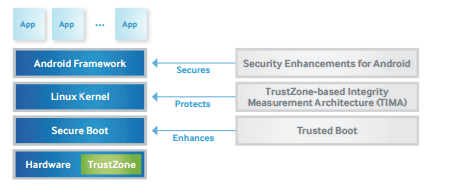
\includegraphics[scale=0.9]{Images/samsung_knox_platform_security}
\caption{Samsung Knox Platform Security}
\end{figure}
In der Grafik links sieht man den groben Aufbau eines Android Systems.In der Grafik rechts sieht man die Technologien, mit deren Hilfe es Samsung möglich ist in die Schichten einzugreifen.
\paragraph{Kerntechnologien der Platform Security}

\begin{itemize}
	\item \textbf{SE for Android}
	\begin{itemize}
		\item \textbf{Funktionsweise} \newline SE for Android basiert auf SELinux-Technologie und definiert die Zugriffskontrolle auf Linux-Ebene. Mandatory Access Control (MAC) und Discretionary Access Control (DAC) überwachen und verwalten welche Dateien und Apps auf das System des Geräts zugreifen können.
		\item \textbf{Sicherheit} \newline SE for Android erzwingt MAC, wobei Apps nur genau die Rechte zugewiesen erhalten, die sie für den Zugriff auf das System des Geräts benötigen. Sollte ein böswilliger Benutzer oder eine bösartige App also Zugriff auf das Gerät erhalten, dann betrifft der Schaden immer nur einen bestimmten Bereich, während die restlichen Bereiche des Geräts geschützt bleiben. \par Wenn SE for Android ausgelöst wird, sendet es eine Präventionsinformationsmeldung an den Benutzer des Geräts, die in der Informationsleiste erscheint. Die Präventionsinformationsmeldung gibt an, welche Anwendung versucht hat, auf Daten des Geräts zuzugreifen, und sie wird die Deinstallation der betreffenden Anwendung empfehlen. Beachten Sie dabei jedoch, dass SE for Android auch von autorisierten Anwendungen ausgelöst werden kann. Dies kann vorkommen, wenn die App einen von dem in der SE for Android-Richtlinie vorgegebenen Pfad verwendet. Wenn dies der Fall ist, sollten Sie die Datei der Sicherheitsrichtlinie entsprechend aktualisieren.
	\end{itemize}
	\item \textbf{ARM TrustZone-Based Integrity Measurement Architecture (TIMA)}
	\begin{itemize}
		\item \textbf{Funktionsweise} \newline TIMA schützt Ihr Gerät auf zwei verschiedene Weisen. Erstens prüft sie in regelmäßigen Abständen, ob der Kernel des Geräts geändert wurde, indem sie den gegenwärtigen Zustand mit dem Original-Kernel vergleicht. Zweitens authentifiziert TIMA Kernel-Module, wenn diese geladen werden, sodass Geräte nie ungeschützt sind.
		\item \textbf{Sicherheit} \newline Die TIMA TrustZone ist ein manipulationssicherer Sektor des ARM-Prozessors in Ihrem Gerät. Sie authentifiziert und verifiziert den Linux-Kernel über regelmäßige Messungen. Wenn TIMA for Android ausgelöst wird, sendet es eine Ermittlungsinformationsmeldung an den Benutzer, die in der Informationsleiste erscheint. In der Meldung werden Sie normalerweise zum Neustart des Geräts aufgefordert.
	\end{itemize}
	\item \textbf{Secure Boot und Trusted Boot}
	\begin{itemize}
		\item \textbf{Funktionsweise} \newline Secure Boot verhindert, dass unbefugte Bootloader und Kernels in das Gerät geladen werden. Dies bedeutet, dass Ihr Gerät nicht manipuliert wurde und der KNOX-Container geladen werden kann. \par Trusted Boot vergleicht den Bootloader und den Kernel des Betriebssystems mit den originalen Werksversionen. Dies wird dadurch erreicht, dass die Originaldaten des Geräts aufgezeichnet werden und das Gerät permanent beim Systemstart mit diesen gegengeprüft wird, um sicherzustellen, dass sich diese Daten nicht geändert haben.
		\item \textbf Sicherheit \newline Es gibt vier Bootloader auf dem Gerät. Jeder Bootloader prüft die Gültigkeit des vorhergehenden Bootloaders oder Kernels. Trusted Boot sichert diese Bootloader. Die Funktion ist in der ARM TrustZone, einem manipulationssicheren Sektor des ARM-Prozessors, eingebettet. Trusted Boot verwendet kryptografische Schlüssel, um sicherzustellen, dass die Messungen am Gerät dem Original entsprechen. Diese Schlüssel werden erst von Trusted Boot freigegeben, wenn SE for Android bestätigt, dass genehmigte Firmware auf dem Gerät ausgeführt wird.
	\end{itemize}
\end{itemize}

\subsubsection{Application Security}
\paragraph{Application Containers}
Container sind quasi ein Android im Android und bezeichnet einen gesicherten, separaten Bereich (Container) auf dem Gerät. Dieser Bereich hat einen eigenen Homescreen, eigene Anwendungen und eigene Daten. Diese Funktion ist damit vergleichbar mit einer Art Dual-Boot-Variante. Anwendungen außerhalb des Containers haben dabei keinerlei Zugriff auf die Daten oder Prozesse innerhalb des Containers. Anwendungen innerhalb des Containers haben grundsätzlich keinen Zugriff auf Daten außerhalb des Containers. 
\par 
Mittels Richtlinienkonfiguration kann der IT-Verwalter des Gerätes einen read-only (nur lesen) Zugriff für bestimmte Anwendungen im Container auf Daten außerhalb des Containers einrichten. Umgekehrt besteht diese Möglichkeit allerdings nicht. Daten innerhalb des Containers werden dabei mit einem Verschlüsselungsalgorithmus und einem AES-256 Bit Schlüssel geschützt. Ein Zugriff ist erst nach Eingabe eines Passwortes möglich.
\paragraph{On-Device Data Encryption (ODE)}
ODE ist ein im Knox enthaltenes Feature zur Verschlüsselung von Daten. Dabei kann sowohl der sichere Container als auch der normale Bereich, sowie interner als auch externer Speicher verschlüsselt werden. Verwendet wird ein AES Algorithmus mit einem 256 Bit starken Schlüssel. Die Verschlüsselungsfunktion kann vom User selbst unter den Einstellungen oder vom IT Administrator durch eine Richtlinie aktiviert werden.
\paragraph{Virtual Private Network Support (VPN)}
VPN-Verbindungen verwendet man um sicherzustellen, dass Daten bei der Übertragung geschützt sind und um den Netzwerkverkehr nicht mit den Daten von persönlichen Apps zu belasten.
\begin{itemize}
	\item \textbf{Funktionsweise} \newline 
	KNOX Workspace bietet 3 VPN-Optionen für den Schutz Ihrer Daten bei der Übertragung. Ein geräteweites VPN kann von Benutzern konfiguriert werden, sofern sie den entsprechenden Servernamen und die dazugehörigen Informationen zur Hand haben. VPN pro App oder ein containerweites VPN kann von IT-Administratoren über die MDM-Konsole eingerichtet werden. Auf der MDM-Konsole kann man bis zu 5 verschiedene VPN-Profile einrichten und diese einzelnen Apps zuweisen, um VPN pro App zu implementieren.
	\item \textbf{Sicherheit} \newline 
	VPN-Verbindungen sind die sicherste Methode, um die Daten bei der Übertragung zu schützen. Der KNOX VPN-Client kann ein bestehendes VPN-Gateway für den Schutz von Daten verwenden. KNOX VPN ist über Ihre MDM-Konsole im FIPS-Modus konfigurierbar. Zu den Sicherheitsfunktionen gehören NSA-Suite-B-Algorithmen, Unterstützung für X.509 mit Zertifikatsprüfung auf OCSP-Basis und 256-Bit-AES-Verschlüsselung. Wenn Ihr Unternehmen SmartCards verwendet, können diese mit VPN-Anmeldedaten konfiguriert werden.
\end{itemize}

\subsubsection{Management}
Mit MDM (Mobile Device Management) bietet Samsung Knox der IT Abteilung des Unternehmens die Möglichkeit eine integrierte Lösung zur Verwaltung und Administration von Samsung-Geräten vorzunehmen, ohne dabei auf Drittanbieter zurückgreifen zu müssen. Der Nachteil dabei ist die ausschließliche Verwendung mit Samsung-Geräten, welche über Samsung Knox verfügen.
\par
Samsung Knox gibt es in 2 Varianten, wobei beide Varianten ein MDM als Basis benötigen um zu funktionieren.
\paragraph{Knox Lösungen}
\begin{itemize}
	\item \textbf{Knox Express} \newline
	Diese Lösung ist für kleine bis mittelständische Unternehmen gedacht. Sie ist gratis, jedoch limitiert auf 250 Geräte. \par Falls die 250 Plätze nicht mehr reichen, kann man Knox Express problemlos auf Knox Premium updaten. \par Das ist die Variante, die die Projektgruppe empfehlen würde, da sie gratis ist und da laut Angaben von der Firma Kapsch es eher unwahrscheinlich ist, dass ein Kunde mehr als 250 Geräte hat und falls doch ist es ja problemlos auf Premium erweiterbar.
	\item \textbf{Knox Premium} \newline
	Diese Komplettlösung eignet sich ideal für Unternehmen, in denen Sicherheit oberste Priorität hat. \par Knox Premium kostet pro Gerät pro Monat 1\$ und kann um zusätzliche Add-ons erweitert werden. \par Weiters bietet Knox Premium einige zusätzliche Features für Android und eine bessere IOS Integration. In Hinblick auf die von Kapsch erwünschten Funktionalitäten bringen diese zusätzlichen Features jedoch keine Vorteile.
	\item \textbf{Add-Ons}
	\begin{itemize}
		\item \textbf{Knox Workspace} \newline
		Knox Workspace ist eine Erweiterung im Bereich Container. \par Dieses Add-on bietet eine einfachere Konfiguration, zwei Container pro Gerät, zusätzliche Apps und verbesserte Sicherheitsfunktionen. \par Die Hauptfeatures, die Workspace mit sich bringt, sind: 
		\begin{itemize}
			\item Erweiterte Containerverwaltung mit sicheren Richtlinien
			\item Datenverschlüsselung bei jedem Entsperren des Containers
			\item Pro-App-VPN für sichere und schnelle Verbindung
			\item Support für zwei separate Container für maximale Produktivität und für Trennung von arbeitsbezogenen und privaten Daten
		\end{itemize}
	All diese Einstellungen, die mit Knox Workspace dazu kommen, gelten nur innerhalb des Containers. Da es jedoch keine Einstellung gibt um zu verhindern, dass der Benutzer den Container verlässt und somit alle Workspace-Einstellungen umgeht, ist dieses Add-on in unserem Fall ungeeignet. \par Jedoch soll in Zukunft eine Art Contaier-only-mode implementiert werden. Sobald dieser vorhanden ist, wäre Knox Worspace auf jeden Fall ein Addon das in Betracht gezogen werden sollte.
		\item \textbf{Knox IAM} \newline
		Knox IAM ist eine SSO-Lösung(Single Sign-On-Lösung). \par Das heißt mit dem IAM Add-on hat man nur mehr einen einzigen Account, mit den man sich in allen Apps anmelden kann.
	\end{itemize}
\end{itemize}
\paragraph{MDMs}
Knox bietet zur Verwaltung der Geräte ein eigenes MDM, das EMM, hat aber auch genügend Partner, deren MDMs Samsung Knox Funktionen implementiert haben. \par
Samsung Knox funktioniert also mit jedem MDM aus der nachfolgenden Liste:
\begin{itemize}
	\item \textbf{Liste an Kompatiblen MDMs}
	\begin{itemize}
		\item Samsung EMM
		\item MobileIron
		\item Absolute Software
		\item AirWatch
		\item CA Technologies
		\item Centrify
		\item Citrix
		\item FancyIron
		\item MaaS360
		\item NQ Mobile
		\item Samsung SDS
		\item SAP
		\item SOTI
	\end{itemize}
	\item \textbf{Samsung EMM} \newline
	Samsung KNOX EMM ist eine cloudbasierte Verwaltungslösung für Unternehmen. IT-Administratoren können damit Benutzer, Apps und plattformübergreifende Geräte über eine cloudbasierte Konsole verwalten. Außerdem bietet KNOX EMM Single Sign-On (SSO) und eine starke Authentifizierung für eine benutzerfreundliche und sichere Arbeitsumgebung für Mitarbeiter. \par Es ist einfach zu installieren und sehr übersichtlich gestaltet. Falls in der Firma noch keine andere MDM Lösung installiert sein sollte, ist EMM zu empfehlen.
\end{itemize}





\chapter{Auswahl \& Konzept}
\section{Endergebnis und Empfehlung}
Nach Abschluss des Evaluierungsprozesses ist das Projektteam an diesem Punkt in der Lage eine Empfehlung an das Unternehmen Kapsch auszusprechen. In diesem Teil wird nun erläutert, welches evaluierte Konzept mit den Anforderungen des Auftraggebers übereinstimmt und wodurch dies zu Stande gekommen ist. Nachdem die Linuxmanipulation aus Garantie technischen Gründen bereits als ausgeschieden gilt, befasst sich der folgende Abschnitt nur mehr mit den Konzepten MDM\footnote{Mobile Device Management}, MDM + Container und Samsung Knox.
\section{Evaluierung}
Um feststellen zu können, welche der 3 Lösungen am besten die Anforderungen des Auftraggebers erfüllen kann, hat das Projektteam eine Nutzwertanalyse erstellt, mit derer Hilfe das Projektteam die Funktionen der Systeme direkt miteinander vergleichen konnten.
\subsection{Nutzwertanalyse}
Die Tabelle auf der folgenden Seite zeigt den Vergleich zwischen Mobile Device Management, Mobile Device Management + Container und Samsung Knox in Form einer Nutzwertanalyse.

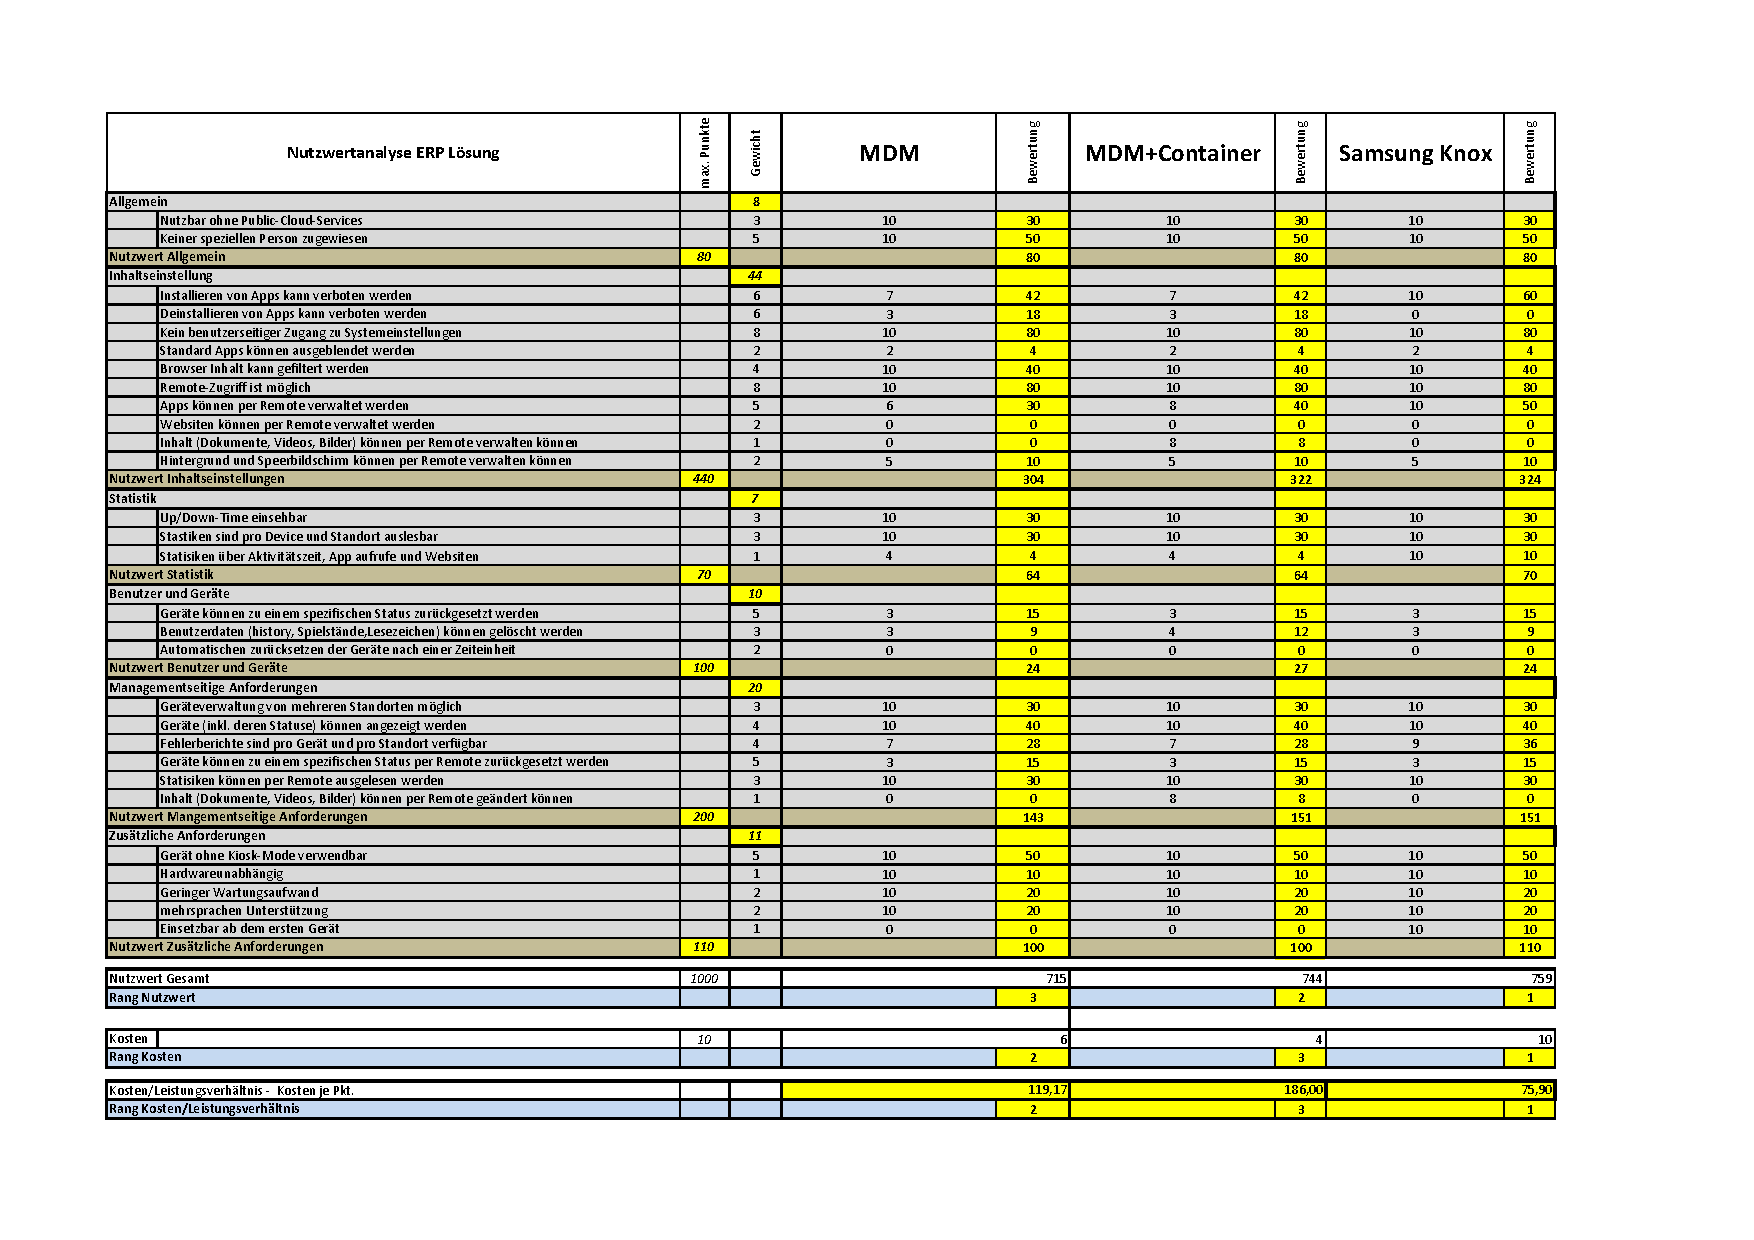
\includepdf[landscape]{nutzwertanalyse}

\section{Auswertung der Evaluierung}
Um ein aussagekräftiges Ergebnis zu erhalten, wurden die Anforderungen des Gesamtsystems in verschiedene Unterpunkte unterteilt, welche auf ihre Funktionstüchtigkeit hin untersucht wurden. \par
Die Lösungen wurden dann je nach Erfüllungsgrad der einzelnen Punkte bewertet, was eine objektive Vergleichbarkeit schaffen sollte.
\subsection{Allgemein}
Da alle drei Systeme sowohl ohne pulic-cloud-service nutzbar waren als auch keiner speziellen Person zugewiesen werden müssen, haben alle drei Lösungen die volle Punkteanzahl erreicht und sind somit, was diesen Punkt angeht, gleich auf.
\subsection{Inhaltseinstellungen}
In diesem Bereich, hat sich herausgestellt, ist Samsung Knox kapp aber doch noch vor der MDM+Container Lösung das am besten geeignete System. Denn auch wenn es mit MDM+Containern möglich ist, die Deinstallation von betriebsinternen Apps zu verbieten und man auch Inhalte der Geräte wie zum Beispiel Bilder, Dokumente, etc per remote verwalten kann, ist Samsung hier die bessere Alternative, da es eine bei weitem bessere Verwaltung von Apps per Remote bietet. \par
Eine Anforderung, die jedoch keines der drei Systeme erfüllen konnte, war das Verwalten von Websiten per remote.
\subsection{Statistik}
Auch den Unterpunkt "Statistiken" kann Samsung Knox wieder für sich entscheiden. Diesmal jedoch mit einem größeren Vorsprung. Zurückzuführen ist das darauf, dass Samsung Knox die Möglichkeit bietet, sich jede beliebige Statistik die man für sein Unternehmen haben will, einfach mittels SQL Code selbst zu erzeugen.
\subsection{Benutzer und Geräte}
In diesem Bereich kann die MDM+Container Lösung punkten. Denn im Gegensatz zu den anderen zwei Systemen, kann man mit dieser Lösung am Gerät gespeicherte Lesezeichen löschen. \par
Auch bei diesem Unterpunkt gibt es wieder eine Anforderung die mit keinem unserer getesteten Systeme umsetzbar war. Und zwar war es nicht möglich die Geräte so zu konfigurieren, dass sie sich nach einer gewissen Zeit von alleine auf einen definierten Stand zurücksetzen.
\subsection{Managementseitige Anforderungen}
Bei der Erfüllung der managementseitigen Anforderungen sind Samsung Knox und die MDM+Container-Lösung gleich auf. Denn den Vorsprung den Knox gewinnt durch besseres Handling der Fehlerberichte, kann die MDM+Container-Lösung dadurch wegmachen, das sie im Gegensatz zu Samsung Knox eine Möglichkeit bietet, Geräteinhalt per remote zu ändern.
\subsection{Zusätzliche Anforderungen}
Da Samsung Knox das einzige System ist, welches bereits ab dem ersten Gerät einsetzbar ist und sonst alle Punkte von allen Systemen erfüllt werden, ist auch hier Knox der klare Sieger.

\section{Empfehlung}
Nach eingehender Analyse ist das Projektteam zu dem Schluss gekommen, dass für die geplanten Projekte der Firma Kapsch die Betriebsplattform Samsung Knox am ehesten geeignet ist. Es implementiert die meisten der benötigten Features, aber lässt dennoch einige fundamentale Punkte aus. Deshalb ist es hier für das Projektteam auch nicht möglich eine hundert prozentige Empfehlung zu geben. Den Informationen der Dokumentation von Samsung Knox zur Folge werden einige benötigte Features in kommenden Versionen eingebaut. Allerdings ist nicht absehbar, ob und wann diese erscheinen. Für die beiden anderen Systeme kann deshalb keine Empfehlung ausgesprochen werden, weil sie besonders im Einsatz mit Nicht-Samsung-Geräten signifikant weniger Funktionen bieten.


\chapter{Ergebnis}
Das Ergebnis unseres erfolgreich abgeschlossenen Projekts setzt sich aus zwei Komponenten zusammen:
\begin{itemize}
	\item Untersuchungsbericht
	\item Prototyp
\end{itemize}
\begin{figure}[H]
\centering
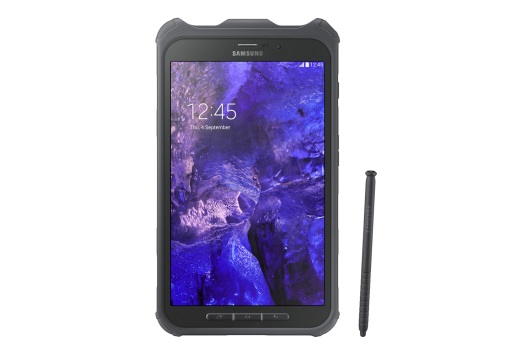
\includegraphics[scale=1.0]{Images/prototyp}
\caption{Der Prototyp}
\end{figure}
Die genauere Definition dieser zwei Komponenten findet man einerseits im Lastenheft, welches wir von unserem Auftraggeber erhalten haben, und andererseits in den von uns vorbereiteten und mit Kapsch abgesprochenen Kriterien, welche in unserem Pflichtenheft abgeklärt wurden. 
\paragraph*{}
Um das Projekt als erfolgreich zu bezeichnen, muss im angesprochenen Untersuchungsbericht ein Vergleich von drei bis vier Softwarelösungen zur Absicherung von Tablets angestellt werden. Zusätzlich müssen zu den jeweiligen Softwarelösungen die diversen Vor– und Nachteile angegeben sein, sowie auch das Fehlen von Einstellungsmöglichkeiten.
\paragraph*{}
Am Ende des Untersuchungsberichts hat ein Vergleich der Systeme zu stehen, aus dem herausgeht, welches, nach der Meinung des Projektteams, eingesetzt werden sollte. Dies muss mit Argumenten bekräftigt werden.
\paragraph*{}
Weiters muss auch der angesprochene Prototyp erstellt bzw. konfiguriert werden. Dieser ist als ein Android–Tablet definiert, welches auf  die Anforderungen eines Beispielunternehmens zugeschnitten ist. Dabei sollen bereits einige Einschränkungen mit der von uns ausgewählten Softwarelösung gemacht worden sein.
\paragraph*{}
Zu diesen Einschränkungen zählt beispielsweise, dass man genau drei bestimmte, vom Auftraggeber festgelegte Apps verwenden darf, dass der Zugang zu den Einstellungen blockiert wird, was bedeutet, dass der User mit dem Tablet nicht in die Einstellungen gehen kann und dort diverse Veränderungen vornehmen kann.
\paragraph*{}
Weiters darf keine Verbindung mit einem Computer im physischen Sinn möglich sein, was bedeutet, dass, falls man das Tablet mit einem Micro USB Kabel an einen Computer anschließt, dieses nicht vom PC erkannt wird und es so nicht verwendet werden kann.
\paragraph*{}
Eine weitere Einschränkung ist, dass man mit dem Tablet keine Apps, Fotos, Videos usw. downloaden können darf.
\paragraph*{}
Die letzte gröbere Einschränkung ist, dass man die gesicherte Umgebung nicht verlassen kann, was bedeutet, dass man die Schutzsoftware nicht ausschalten und das Tablet für seinen privaten Gebrauch verwenden kann.
\paragraph*{}
Sollten diese Kriterien sowohl von unserem Prototypen, als auch von unserem Untersuchungsbericht erfüllt und von Kapsch akzeptiert werden, so erhält dieses Projekt den Status „ERFOLGREICH ABGESCHLOSSEN!“. 
\chapter{Lessons Learned}
\section{Sebastian Götze}
Durch das Diplomprojekt Kapsch Tablet Infrastructure habe ich gelernt, dass es besonders bei der Recherche wichtig ist, sich nicht immer auf den Inhalt von Dokumenten und Präsentationen zu verlassen, weil dieser oft nicht die Realität wiederspiegeln. Besonders beim System Samsung Knox hat sich dies deutlich herauskristallisiert, da in Samsungs Unterlagen zwar steht, dass es einen Modus gibt, in dem der Nutzer sich ausschließlich in einem abgesicherten Container befindet, aber dieser in der Praxis nur bedingt existiert. Der Modus war vorhanden, allerdings war es für den Nutzer jederzeit möglich aus diesem herauszuspringen. Ein weiterer wichtiger Lernaspekt für mich war es, dass man bei der Installation von unbekannten Systeme vor Beginn die Installationsanleitung lesen sollte und nicht sich danach auf Fehlersuche zu begeben. Besonders bei der Einrichtung der zusätzlichen Containerapplikationen zu MobileIron wäre dies von Vorteil gewesen, da es hier einige wichtige Details zu beachten gab, ohne die der Prozess nicht abgeschlossen werden konnte.
\section{Samuel Hammer}
Während das Projekts KTI habe ich in erster Linie vieles bezüglich Projektmanagement gelernt. Durch die oftmals eng gesetzten Zeitintervalle, war es äußerst wichtig die Koordination zwischen den zwei Subteams bzw. den einzelnen Teammitgliedern zu perfektionieren. 
Ein teilweise großes Problem war auch, dass sich Projektbezogene Abgaben und Termine immer wieder mit Tests, Schularbeiten und anderen unterrichtsbezogenen verpflichtungen überschnitten. Hier war es von großer wichtigkeit, sich mit den zuständigen Lehrern bzw. dem Projektpartner abzusprechen. 
Einiges gelernt habe ich natürlich auch in Hinblick auf die wichtigen Dokumente, welche es im Laufe des Projektes zu erstellen und aktualisieren gab.
Alles in Allem war das Projekt "Kapsch Tablet Infrastructure" eine wertvolle Erfahrung, aus der ich viel für meine zukünftige berufliche Laufbahn mitnehmen werden.

\newpage

\section{Michael Kaufmann}
Einer der wichtigsten Punkte die ich durch die Arbeit am Diplomprojekt in Erfahrung bringen konnte ist, wie wichtig gut funktionierende Kommunikation innerhalb des Projekt Teams ist. Um den Arbeitsaufwand bestmöglich zu verteilen und um, so produktiv wie möglich, sein zu können haben wir Sub-Teams gebildet und unser Projekt in technischen und dokumentationsbezogenen Teil geteilt.
Das Problem hierbei war nur das die Sub-Teams teilweise abhängig von einander waren und es hin und wieder vorkam das die Arbeit, auf die das eine Team warten musste um weiter machen zu können, bereits erledigt war, aber diese nichts davon wussten. Dies führte logischerweise zu Verzögerung des gesamten Projekts. 
Außerdem habe ich gelernt dass man der Dokumentation und den Whitepapers einer Fertiglösung nicht immer blind vertrauen kann. Denn wie zum Beispiel im Falle Samsung knox sich herausgestellt hat, werden oft Funktionen versprochen, welche tatsächlich nicht existieren. Dies führt nicht nur zu einer Verzögerung des Aufwandes was das testen der Lösung betrifft, sondern auch dazu das die Lösung vor dem Testen besser eingeschätzt wurde als sie tatsächlich war.

\section{Konstanze Müller}
Das diesjährige Diplomprojekt mit unserem Partner der Kapsch Business Com gewährte mir in erster Linie einen Einblick eines kompletten Projektdurchlaufes in der Praxis. Theoretische Inhalte für einen reibungslosen Projektverlauf, welche wir in den Jahren davor im Unterricht gelehrt bekommen haben, konnten wir als Projektteam in diesem Abschlussjahr erfolgreich umsetzen. Auch wenn unser Projektleiter Philip Steinhäuser in diesem Bereich die Oberhand hatte, unterstütze ich ihn so gut wie möglich und war somit auch mit formalen Abwicklungskriterien vertraut. 
Aus Projekttechnischer Sicht lernte ich, dass man den Aufwand für die Evaluierung von einem System schwer im Voraus abschätzen kann. Des Öfteren war es der Fall, dass Anforderungen von der Checkliste nicht auf Anhieb funktionierten. Selbstverständlich hört man nicht gleich auf zu testen, sondern probiert weiteres. Das Schwierige meiner Meinung war nun den richtigen Zeitpunkt zu finden, um mit einer hohen Wahrscheinlichkeit sagen zu können, dass diese Anforderung vom ausgewählten System nicht unterstützt wird. In Summe bedeutet dies, dass man in Projekten wie diesem sich selbst eine Grenze stecken muss um auch ein schlussendliches Ergebnis vorlegen zu können. 

\section{Philip Steinhäuser}
Für mich als Projektleiter hat dieses Projekt ein Menge an Erfahrungen  nicht nur im Managementbereich sondern auch im Zwischenmenschlichen Umgang bereitgehalten, da ich in einigen Situationen dazu gezwungen war ein Machtwort zu sprechen wenn es Streitigkeiten innerhalb des Projektteams gegeben hat. Zusätzlich hab ich einiges zum Thema Zeitplanung und Terminkoordination gelernt, was mir auf meinem weiteren Weg welcher mich hoffentlich in die Wirtschaft bzw. einen wirtschaftlichen Beruf führen wird helfen wird. Zu guter Letzt bleibt mir nicht mehr zu sagen als das ich dieses Projekt als ein für mich sehr Erfahrungsreiches Ereignis verbuche, welches mir in den Bereichen der Teamführung bzw. Projektleitung oder Projektcontrolling sowie Projektmanagement als auch Krisenmanagement eine bzw. mehrere Lehrstunden erteilt hat. Dennoch möchte nichts was wir an dem Projekt gemacht haben sowie die Zusammenarbeit mit diesem großartigen Projektteam missen.
\chapter{Danksagung}
Wir möchten uns in erster Linie bei unseren Betreungslehrern, Herrn DI Harald Swoboda und Herrn DI Hannes Färberböck für die großartige Unterstützung während des gesamten Projektverlaufs bedanken.
\paragraph*{}
Großer Dank gilt auch Herrn DI (FH) Mag. Bernhard Bruckner und \newline Herrn Jürgen Krammer, die uns im Namen der Kapsch BusinessCom bei Problemen immer mit Rat und Tat zur Seite standen.
\paragraph*{}
Herzlichen Dank auch an unsere Deutsch Professorin, Frau Dr. Margareth Antonescu, die sich freundlicherweise dazu bereit erklärte, diese Diplomarbeit zu korrigieren.




\chapter{Quellenverzeichnis}
\printbibliography[heading=bibintoc]
\chapter{Abbildungsverzeichnis}
\listoffigures
\chapter{Tabellenverzeichnis}
\listoftables


\chapter{Begleitprotokoll}
\textbf{Name des Schülers:} Sebastian Götze \newline
\textbf{Name des Schülers:} Samuel Hammer \newline
\textbf{Name des Schülers:} Michael Kaufmann \newline
\textbf{Name der Schülerin:} Konstanze Müller \newline
\textbf{Name des Schülers:} Philip Steinhäuser
\newline
\newline
\textbf{Thema der Arbeit:} KTI - Kapsch Tablet Infrastructure
\newline
\newline
\textbf{Name der Betreuungsperson:} DI Harald Swoboda \newline

\newpage

\begin{table}
	\centering
	\begin{tabular}{| c | c | p{6cm} | p{4cm} |}
		\hline
		\textbf{Datum} & \textbf{Bearbeiter/in} & \textbf{Tätigkeit} & \textbf{Anmerkung}
		\\\hline %----------new line----------
		26.01.2015 
		&%-----
		Philip Steinhäuser
		&%-----
		\begin{itemize}
			\item Kurzfassung in Deutsch
			\item Kurzfassung in Englisch
		\end{itemize}
		&%-----
		\\\hline %----------new line----------
		26.01.2015
		&%-----
		Samuel Hammer
		&%-----
		Beginn der Android-Studie
		&%-----
		Erste Teile der Diplomarbeit in LaTeX integriert.
		\\\hline %----------new line----------
		27.01.2015
		&%-----
		Philip Steinhäuser
		&%-----
		Einleitung erstellt
		&%-----
		\\\hline %----------new line----------
		27.01.2015
		&%-----
		Samuel Hammer
		&%-----
		einleitung in LaTeX Dokument integriert
		&%-----
		\\\hline %----------new line----------
		29.01.2015
		&%-----
		Philip Steinhäuser
		&%-----
		Ergebnis aktualisiert
		&%-----
		\\\hline %----------new line----------
		29.01.2015
		&%-----
		Samuel Hammer
		&%-----
		Weitere Teile in LaTeX eingebunden
		&%-----
		\\\hline %----------new line----------
		19.02.2015
		&%-----
		Samuel Hammer
		&%-----
		Aktualisierung der Studie
		&%-----
		\\\hline %----------new line----------
		04.03.2015
		&%-----
		Philip Steinhäuser
		&%-----
		Aktualisierung der Struktur der Diplomarbeit (Inhaltsverzeichnis)
		&%-----
		\\\hline %----------new line----------
		27.03.2015
		&%-----
		Samuel Hammer
		&%-----
		Aktualisierung der Struktur der Diplomarbeit (Inhaltsverzeichnis)
		&%-----
		\\\hline %----------new line----------
		02.04.2015
		&%-----
		Samuel Hammer
		&%-----
		\begin{itemize}
			\item Anlegen der Punkte Varianten und Auswahl \& Konzept
			\item Aktualisierung des Quellenverzeichnisses
		\end{itemize}
		&%-----
		\\\hline %----------new line----------
		16.04.2015
		&%-----
		Philip Steinhäuser
		&%-----
		Übertragung des Inhaltes des Untersuchungsberichts in den Punkt Varianten.
		&%-----
		\\\hline %----------new line----------
		16.04.2015
		&%-----
		Samuel Hammer
		&%-----
		Übertragung des Inhaltes des Untersuchungsberichts in den Punkt Auswahl \& Konzept
		&%-----
		\\\hline %----------new line----------
		30.04.2015
		&%-----
		Samuel Hammer
		&%-----
		Aktualisierung der Struktur der Diplomarbeit (Inhaltsverzeichnis)
		&%-----
		\\\hline %----------new line----------
		30.04.2015
		&%-----
		Philip Steinhäuser
		&%-----
		Vervollständigung der Diplomarbeit
		\begin{itemize}
			\item Text zu Projektpartner verfasst
			\item Arbeitsaufteilung dokumentiert
			\item Lessons Learned verfasst
			\item Danksagung hinzugefügt
			\item Quellen-, Tabellen- und Abbildungsverzeichnis aktualisiert
		\end{itemize}
		&%-----
		\\\hline %----------new line----------
		30.04.2015
		&%-----
		Samuel Hammer
		&%-----
		Vervollständigung der Diplomarbeit
		\begin{itemize}
			\item Text zu Projektpartner verfasst
			\item Arbeitsaufteilung dokumentiert
			\item Lessons Learned verfasst
			\item Danksagung hinzugefügt
			\item Quellen-, Tabellen- und Abbildungsverzeichnis aktualisiert
		\end{itemize}
		&%-----
		\\\hline %----------new line----------
	\end{tabular}
	\caption{Begleitprotokoll}
\end{table}

\include{Kapitel/anhang}

\end{document}


